\documentclass[final, 1p, times]{elsarticle}

% Keep only essential packages
\usepackage{amsmath}
\usepackage{amssymb}
\usepackage{adjustbox}
\usepackage{booktabs}
\usepackage[table]{xcolor}
\usepackage{graphicx}
\usepackage{setspace}
\usepackage{hyperref}
\usepackage{longtable}
\usepackage{threeparttable}
\usepackage{subcaption}
\usepackage{colortbl}
\usepackage{multirow}

% Bibliography setup for elsarticle
\usepackage[numbers]{natbib}

\begin{document}

\begin{frontmatter}

\title{Raising EPC Standards: A Triple Win Strategy for the UK Housing Market and Reaching Net-Zero}

% Author information
\author[oxford]{Charlotte Wargniez}
\ead{charlotte.wargniez@lincoln.ox.ac.uk}
\author[oxford]{Quentin Coutellier}
\author[glasgow]{Hormoz Ramian}

% Affiliations
\affiliation[oxford]{organization={School of Geography and the Environment, University of Oxford},
                     country={UK}}
\affiliation[glasgow]{organization={Adam Smith Business School, University of Glasgow},
                      country={UK}}



\begin{abstract}
This paper employs a microeconomic approach to estimate the impact and cost of imposing Minimum Energy Efficiency Standards (MEES) of Band C on the housing sectors in England and Wales. Using an empirical investigation that leverages historical transaction prices, energy performance certificates (EPCs) from 2008-2022, and active listings from 2016-2022, the study estimates an average XXX£ per household, up to £XXX nationwide. While the study suggests property owners could capture green premiums from increased energy efficiency at point of sale, which may compensate some of the large upfront costs associated with retrofitting to a higher standard, we estimate that up to 500,000 privately rented dwellings may be at risk of not being unable to comply with the new policy. Using listing data to empirically measure the effect of such a change in supply in the market, we conclude that a sell off could potentially be leading to an 11\% increase in housing affordability. This would suggest that harnessing market dynamics to achieve net-zero homes by 2050 through higher energy efficiency standards could result in increased efficiency and lower carbon footprint, increased affordability, and a reshuffling in property ownership.
\end{abstract}

\begin{keyword}
Energy efficiency \sep Green premium \sep Housing market \sep Net-zero \sep EPC standards \sep MEES \sep UK housing policy
\end{keyword}

\end{frontmatter}

% Main content sections
\section{Introduction}

The UK's housing sector is at a critical crossroads, facing a multitude of challenges that are deeply intertwined with the nation's broader socio-economic and environmental goals. Among these challenges, the need to decarbonize the housing stock to meet Net Zero commitments by 2050 stands out as a pivotal issue. A significant portion of the UK’s residential buildings, particularly those in the rental sector, are currently underperforming in terms of energy efficiency since as of 2022, homes with an Energy Performance Certificate (EPC) rating above Band C only represented 42\% and 37\% of the total stock in England and Wales, respectively \cite{office_for_national_statistics_age_2022}. This underscores the vast potential—and necessity—for improvements in the energy performance of the UK’s housing stock.\\

In the 2024 elections’ manifesto, the Labour Party mentioned its intentions to invest an additional £6.6 billion over the current parliament to increase home energy efficiency as part of its 'Energy Independence Act' \cite{noauthor_make_nodate} as part of their plan to take increasing actions to reduce energy poverty and increase UK home energy efficiencies in their pursuit of achieving NZ \cite{scott_kings_2024}. This follows decades of multiple policy agendas that have been unsuccessful at engaging privately rented dwellings to improve their energy efficiency \cite{hope_attitudes_2014}. In October 2021, the UK Government released the Heat and Buildings Strategy, outlining its approach to decarbonizing homes and buildings \cite{department_for_energy_security_and_net_zero_desnz_and_department_for_business_energy_and_industrial_strategy_beis_heat_2021}. A primary objective of this strategy is to enhance the energy efficiency of as many homes as possible across England and Wales, with the goal of achieving an EPC rating of Band C by 2035, provided this is practical, cost-effective, and financially viable. Additionally, the strategy aims for as many fuel-poor homes as reasonably practicable to reach an EPC Band C by 2030. While there are existing minimum energy efficiency standards (MEES) for privately and social-rented homes in the UK and Wales \cite{rowe_housing_2024}, new and existing private tenancies were required to be certified as Band E or higher since April 2018 and 2020, respectively (The Energy Efficiency (Private Rented Property) (England and Wales) Regulations, 2015). Should landlords fail to achieve MEES, they may be required to pay a fine up to £5,000 \cite{department_for_energy_security_and_net_zero_2023_2023}. While the UK government does offer grants to partly cover the costs of retrofitting a dwelling up to standards, such as the Boiler Upgrade scheme which subsidises the deployment of heat pumps, and no property owner is currently obligated to spend in excess of £3,500 on reaching the MEES \cite{department_for_energy_security_and_net_zero_2023_2023}. In other words, when a property is unable to reach the MEES within the given expenses, landlors must only make improvements up to that amount \cite{department_for_energy_security_and_net_zero_2023_2023}.   In September 2020 and January 2021, the government consulted whether to amend the current MEES to Band C by 2025 for new leases and 2028 for existing ones and revise upward the £3,500 threshold \cite{department_for_energy_security_and_net_zero_desnz_and_department_for_business_energy_and_industrial_strategy_beis_heat_2021}. In September 2023, then Prime Minister Rishi Sunak announced that the target for UK rented homes would be scratched,  which was later brought back by the Labour Party \cite{noauthor_make_nodate}.\\


Retrofitting homes has been referred to as the most significant challenge to meet the UK Net Zero goals  \cite{alabid_review_2022, uk_green_building_council_ukgbc_retrofit_2021}. As with all infrastructural transformations, sustainable structural retrofits are difficult to implement at a rapid and large scale due to structural, technical and behavioural path dependences \cite{dauda_understanding_2022}. Committing to green retrofits to limit energy consumption and resulting carbon emissions has been not only historically difficult \cite{lowe_technical_2007, chaves_building_2017}, but also complicated due in part to UK property law which acts as an additional barrier for dwellings with mixed tenures and leaseholders (particularly flats) as it requires consent from all stakeholders involved \cite{weatherall_property_2018, bright_exploring_2019}. This is further exacerbated by properties' long lifetime and slow retrofitting rates, making it difficult and costly for the housing sector to shift from its high-emitting paradigm, as it is estimated that nearly 80\% of properties were built to standard levels below those required to meet  Net Zero targets \cite{warren_can_2024, uk_green_building_council_ukgbc_retrofit_2021}. \\

While incentives to commit to expensive retrofits are mixed, there is evidence that mandatory energy efficiency disclosure have resulted in green premiums, increased energy investments, and helped correct some marker failures in the housing sector \cite{cassidy_how_2023, myers_mandatory_2022}. Green Premiums in particular have been extensively studied as consumer’s willingness-to-pay for homes with higher energy efficiency at the time of purchase \cite{harrison_hedonic_1978, bisello_measuring_2020, dalton_green_2018, ghosh_homebuyers_2024, fuerst_is_2020, kahn_capitalization_2014} or rent \cite{bruegge_does_2016, galvin_rental_2023, sieger_inefficient_2023}. While most empirical results concur green premiums on rent and sales prices to be positive (usually around 6\% and 7.6\%, respectively), there are mixed interpretations about the cost-effectiveness of undergoing energy efficiency improvements for landlords \cite{dalton_green_2018}. This is especially the case for deep retrofitting costs which may have long and unpredictable pay-back periods, at the time of resale. Nearly 28\% of all property owners refusing to retrofit do not do so because of the high costs of retrofitting \cite{office_for_national_statistics_age_2022}. It is important to note that estimating these green premiums suffers from confounding factors such as increased demand for homes outpace the supply of newly built homes in the UK \cite{aldridge_housing_2018, nazir_comparison_2020}, and this widening supply gap exacerbates housing shortages, contributing to rising property prices \cite{green_policies_2017}. COVID-19 has also exacerbated the housing crisis, as demand for bigger properties which could accommodate for remote working increased, even well after the pandemic \cite{schwartz_covid-19s_2023}. The resulting housing instability and inaccessibility have far-reaching implications, affecting socio-economic, political, and health systems \cite{murphy_housing_2024, bone_neoliberal_2014, banks_house_2010, mckee_generation_2020}. A notable consequence of this crisis is the decline in housing mobility, particularly among younger generations, which has led to a sharp increase in inequality and reduced disposable income \cite{howard_seven_2024}. This trend is expected to persist, further deepening disparities in the housing market and willingness to commit to green retrofits \cite{green_policies_2017, sabater_age_2023}. \\

In parallel with the housing supply crisis, the private renting sector has expanded rapidly over the past two decades \cite{field_reappraising_2014, bailey_poverty_2020}. As of 2022, approximately 4.6 million households, or 19\% of tenures, were in the private rental sector in England \cite{department_for_levelling_up_housing_and_communities_dluhc_english_2022}. Despite the recent trends in unaffordability, there is a still an ever-increasing demand for properties as people continue to want to own their own homes \cite{aldridge_housing_2018}. A significant proportion of these private renters—over 62\%, equating to around 2.8 million households—expressed plans to buy a home in the future, a notable increase from 56\% in 2019/20 \cite{department_for_levelling_up_housing_and_communities_dluhc_english_2022}. Private renters often face additional challenges, including higher costs for utilities as over half of private renters pay their gas bills via direct debit, and two-thirds do the same for electricity (EHS, 2022). The most common type of tenancy in the domestic sector is a short-hold tenancy (EHS, 2022) leading to increased insecurity amongst the younger and lower-income groups \cite{mckee_generation_2020}. Moreover, private renters generally live in homes with poorer energy performance compared to social renters, further compounding their financial burdens and quality of living (EHS, 2022). \\


Overall, the residential sector is a significant contributor to the UK's energy consumption and carbon emissions since UK households consume on average 3,500 kWh of electricity and 12,000 kWh of gas annually \cite{department_for_business_energy__industrial_strategy_dbeis_energy_2022}. A substantial portion of these emissions stems from heating and electricity use within homes, which are primarily driven by fossil fuels. Notably, space heating accounts for about 63\% of household energy consumption, while water heating, lighting, and appliances collectively contribute to the remaining 37\% \cite{palmer_united_2014}. Energy prices have fluctuated considerably in recent years, with significant increases observed during periods of geopolitical instability, such as the Russian invasion of Ukraine which exacerbated energy price volatility as Europe faces simultaneous disruptions in gas supply and a shift towards alternative energy sources, including renewables \textbf{(Drax Group, 2023)}. The penetration of renewables in the UK grid has been a crucial factor in buffering these price shocks, with renewables accounting for 40\% of electricity generation in 2022, up from 29\% in 2017 \textbf{(National Grid ESO, 2023)}. Retrofitting strategies have shifted from energy conservation measures (i.e., improving wall insulation and double-glazed windows) towards integrating smart technology measures to enhance energy efficiency and integration of renewable technologies \cite{ejidike_global_2023}. Space heating and hot water are responsible for most of the energy consumption in UK households and have hence been considered promising avenues for end-user decarbonization \cite{lowe_technical_2007, kesicki_costs_2012}. Despite being a hard-to-abate sector, reducing end-use emissions associated with heating and powering the domestic building stock seems the most cost-effective measure \cite{kesicki_costs_2012, royapoor_towards_2023}. Technical predictive scenarios have suggested the necessary CO2 emission reductions could be achieved through technology readily available when accompanied by the decarbonization of the system-level electric grid and increasing switch away from fossil fuels \cite{lowe_technical_2007, kesicki_costs_2012, miu_simple_2018}. However, the current retrofitting rates are far below the expected levels to reach NZ targets. Hence, there is an increasing need for policies to enable technological uptake within domestic dwellings if the UK is to meet its net zero targets \cite{wang_innovative_2022, miu_simple_2018}. \\

Heightened concerns regarding the net effect of climate change on domestic energy usage has also led to increased interest in energy conservation and preventative measures to mitigate the anticipated rise in insulation and air-conditioning needs \cite{de_cian_households_2019, poritt_scopus_2012}. In these scenarios, financial motivations, particularly the payback period and projected energy savings, often dominate the decision to renovate, suggesting a "double-win" strategy that reduces both energy costs and carbon emissions \cite{joint_research_centre________________________________________european_commission_building_2020}. The effectiveness of energy efficiency labels to affect property prices has been shown to vary by climatic conditions \cite{taltavull_de_la_paz_green_2019} and age of target audience \cite{wilhelmsson_how_2023}, further adding to the heterogeneous and unpredictable returns from the perspective of property owners. The cognitive perceptions and financial situation of homeowners may significantly impact what is considered a cost-effective energy renovation \cite{galassi_role_2017, ud_din_assessing_2023, wilson_why_2015}. Overall, for homeowners to commit to green retrofits, their preferences and values must align with their perceived financial returns on investment, in that they must be able to expect either an increase in the future sale price and/or a reduction in operational costs (i.e., energy bills) over a sufficiently short pay-back period \cite{wilson_why_2015, wang_holistic_2022}, which results in a demographically and geographically heterogenous decision-making landscape \cite{pelenur_motivations_2014}. \\ 


This study contributes to the ongoing discourse on housing policy and energy efficiency by providing a nuanced understanding of how imposing EPC standards might influence the UK housing market. This research offers insights into how such regulations could not only help achieve environmental targets but also address housing supply and affordability issues. Through detailed empirical analysis, this study aims to inform future policy decisions, ensuring that the UK can meet its Net Zero goals while also fostering a more equitable and efficient housing market. \\

The contributions to the literature are threefold. First, this study provides an empirical estimation of the costs of retrofitting and their associated impact on energy consumption, carbon emissions and overall energy rating. Second, this study attempts to quantify the green premium associated with higher energy ratings as stated in their Energy Performance Certificate (EPC) at point of sale using transaction data. Third, the study estimates the potential effect of an increase on the supply side on property prices using listing data. \\

The remainder of this paper is structured as follows. The next section describes the different datasets used in this study. The third section presents the methodology alongside the main results. Section 4 concludes. 



\section{Data}
Empirical data for this study was collected from three sources, including two open datasets that are historical records of transactions in the UK\footnote{\textit{HM Land Registry: Price Paid Data}. (2016). [Dataset]. \href{https://www.gov.uk/government/collections/price-paid-data}{https://www.gov.uk/government/collections/price-paid-data}} and Energy Performance Certificates (EPCs) of private domestic dwellings in the UK and Wales\footnote{\textit{Energy Performance of Buildings Data England and Wales}. (n.d.). [Dataset]. Retrieved 16 August 2024, from \href{https://epc.opendatacommunities.org/}{https://epc.opendatacommunities.org/}}; as well as aggregated listing data provided by Zoopla. \footnote{Zoopla Limited, © 2024 2. Zoopla Limited. Economic and Social Research Council. Zoopla Property Data, 2024 [data collection].}
The first two datasets were consolidated and matched by unique property identifiers, called Unique Property Reference Numbers (UPRNs), and two mapping files were downloaded from the University of Glasgow Urban Big Data Centre (UBDC), namely the Price Paid Data to UPRNs \footnote{Urban Big Data Centre (2023). Price paid data to UPRN lookup [Data set]. University of Glasgow. \url{https://doi.org/10.20394/agu7hprj}} and the EPC Individual lodgement identifier (LMK) to UPRNs \footnote{Urban Big Data Centre (2023). Energy Performance Certificate to UPRN lookup [Data set]. University of Glasgow. \url{https://doi.org/10.20394/okfrrz60}}. The linkages above provided an accuracy rate of 96\% \cite{urban_big_data_centre_price_2023}. Outliers occurred where the parent UPRNs (e.g. entire building with a unique address) were not distinct from their child UPRNs (e.g. flats in the building) which resulted in anomalistic amounts of transactions. These occurrences were removed during the data cleaning. The data processing for this study was conducted using RStudio, an integrated development environment (IDE) for R. RStudio was chosen due to its comprehensive suite of tools for data manipulation, statistical analysis, and visualization.

\subsection{Energy Performance Certificates}
\label{EPC_data}
Energy Performance Certificates (EPCs) were introduced in the UK on 1 August, 2007 by the Housing Act 2004 and EPBR 2007. \footnote{The Energy Performance of Buildings (Certificates and Inspections) (England and Wales) Regulations 2007}  Figure \ref{fig:EPC_example} below represents the energy efficiency from a typical certificate processed for this study . 
\begin{figure}[h!]
    \centering
    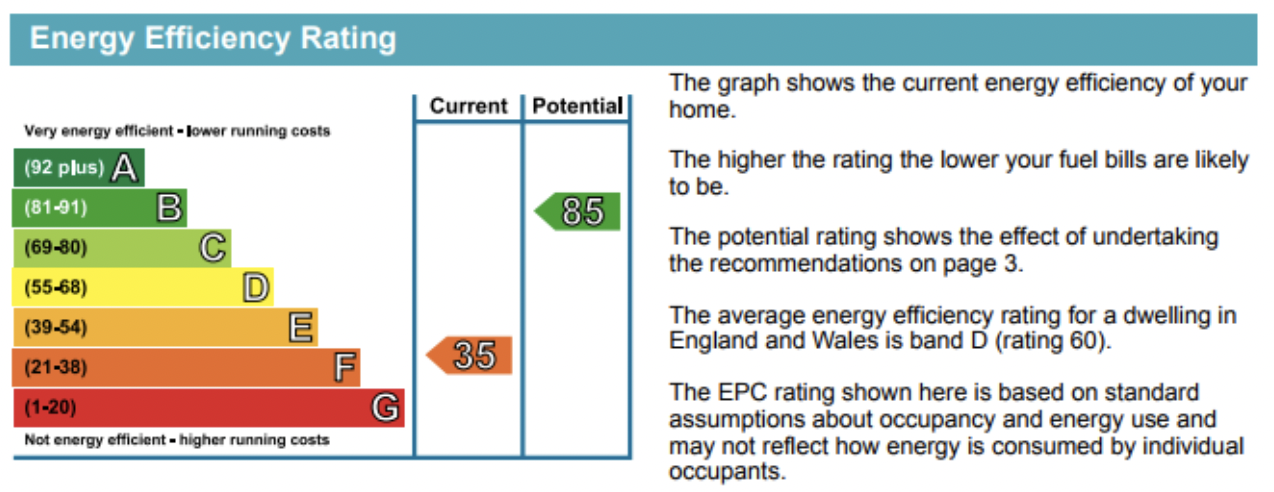
\includegraphics[width=1\linewidth]{src/figures/EPCertificate.png}
    \caption{Typical example of Energy Efficiency Rating reported in an EPC.}
    \label{fig:EPC_example}
\end{figure}
EPCs are determined for a dwelling upon inspection using the Standard Assessment Procedure (SAP). The SAP and RdSAP (Reduced SAP) methodologies are developed by an external organization - the Building Research Establishment (BRE) - and have been criticised for estimating the cost-efficiency - rather than energetic performance - of buildings \cite{kelly_building_2012}. Since SAP ratings mostly take into account energy appliances and house geometry (as estimators of energy use) \cite{department_for_communities_and_local_government_guide_2017, bre_group_standard_nodate} they can overlook the 'fabric' energy efficiency \cite{bolton_energy_2024} \footnote{refers to passive characteristics of buildings which affect energy efficiency, such as insulation} of buildings and may hence not act as the most efficient predictors of carbon emissions \cite{stone_key_2014}. Studies comparing smart meters and domestic EPC energy use ratings have also shown discrepancies in estimations, specially significant over-predictions of energy use in lower rated dwellings due to assumptions on building characteristics and occupancy in the SAP modelling \cite{few_over-prediction_2023}. Other findings suggest this 'measurement error' results in less-accurate estimations in Bands C and lower due to the increase variance in repeated measurements \cite{crawley_quantifying_2019}. Energy-poor properties tend to be the most significantly impacted by the lack of consistency and accuracy of EPC ratings. To avoid these errors, some studies restricted their sample to Bands D and above \cite{ghosh_homebuyers_2024} when attempting to estimate consumer's willingness to pay for energy efficiency. However, this study aims to explore the inequalities and aggregate impacts of improving the housing sector to their maximum potential energy efficiency, which inevitably will affect the lower-rated dwellings. Additionally, when estimating the green premium (see \ref{Sec:green_premium} ) of green-labelled dwellings, it has been shown that government endorsement, simplicity, and financial incentives are key factors determining the trust in certificates rather than the accuracy of the latter \cite{banerjee_eco-labeling_2003, mutter_increasing_2012, martiskainen_role_2019}. Therefore, while there are shortcomings to the SAP methodology, its wide application serves a consistent and standardized index of energy use, sufficient for the purpose of investigating market responses to consumer awareness and policy-incentives. \\


The energy efficiency ratings of 15 million dwellings were extracted from Energy Performance Certificates (EPC) available on the Energy Performance of Buildings Register ('the register' ). Since 2008, all properties listed for sell, rent, or newly constructed must undergo an inspection \cite{department_for_communities_and_local_government_guide_2017}. A certified assessor assigns an energy efficiency ratings from the Standard Assessment Procedure (SAP) in newly built homes and Reduced SAP (RdSAP) in retrofitted homes \cite{department_for_energy_security_and_net_zero_and_department_for_business_energy__industrial_strategy_standard_2013, department_for_energy_security_and_net_zero_and_department_for_business_energy__industrial_strategy_standard_2023}. SAP energy ratings are determined from an estimated ratio of energy consumption and production for each property and provide an energy cost factor on a scale of 1 to 100 (or above 100 if a site generates more energy than it needs) \cite{bre_group_standard_nodate, bolton_energy_2024}. The given numerical scores can be converted to ABCDG bands of energy efficiency - from least efficient and high running costs (1-20 : G) to most energy efficient and low running costs (92+ : A). EPCs provide additional information on the insulation and efficiency of all elements of the property, heating methods, estimated energy needs/costs, and carbon emissions, as well as more detailed information about the properties (such as property size, building age and other property characteristics). After selecting for the observations that could improve their EPC and cleaning the dataset, $15,602,800$ dwellings were kept and analysed as they were able to reach the minimum EPC rating standards imposed by the PRS.

\begin{figure}[h!]
    \centering
    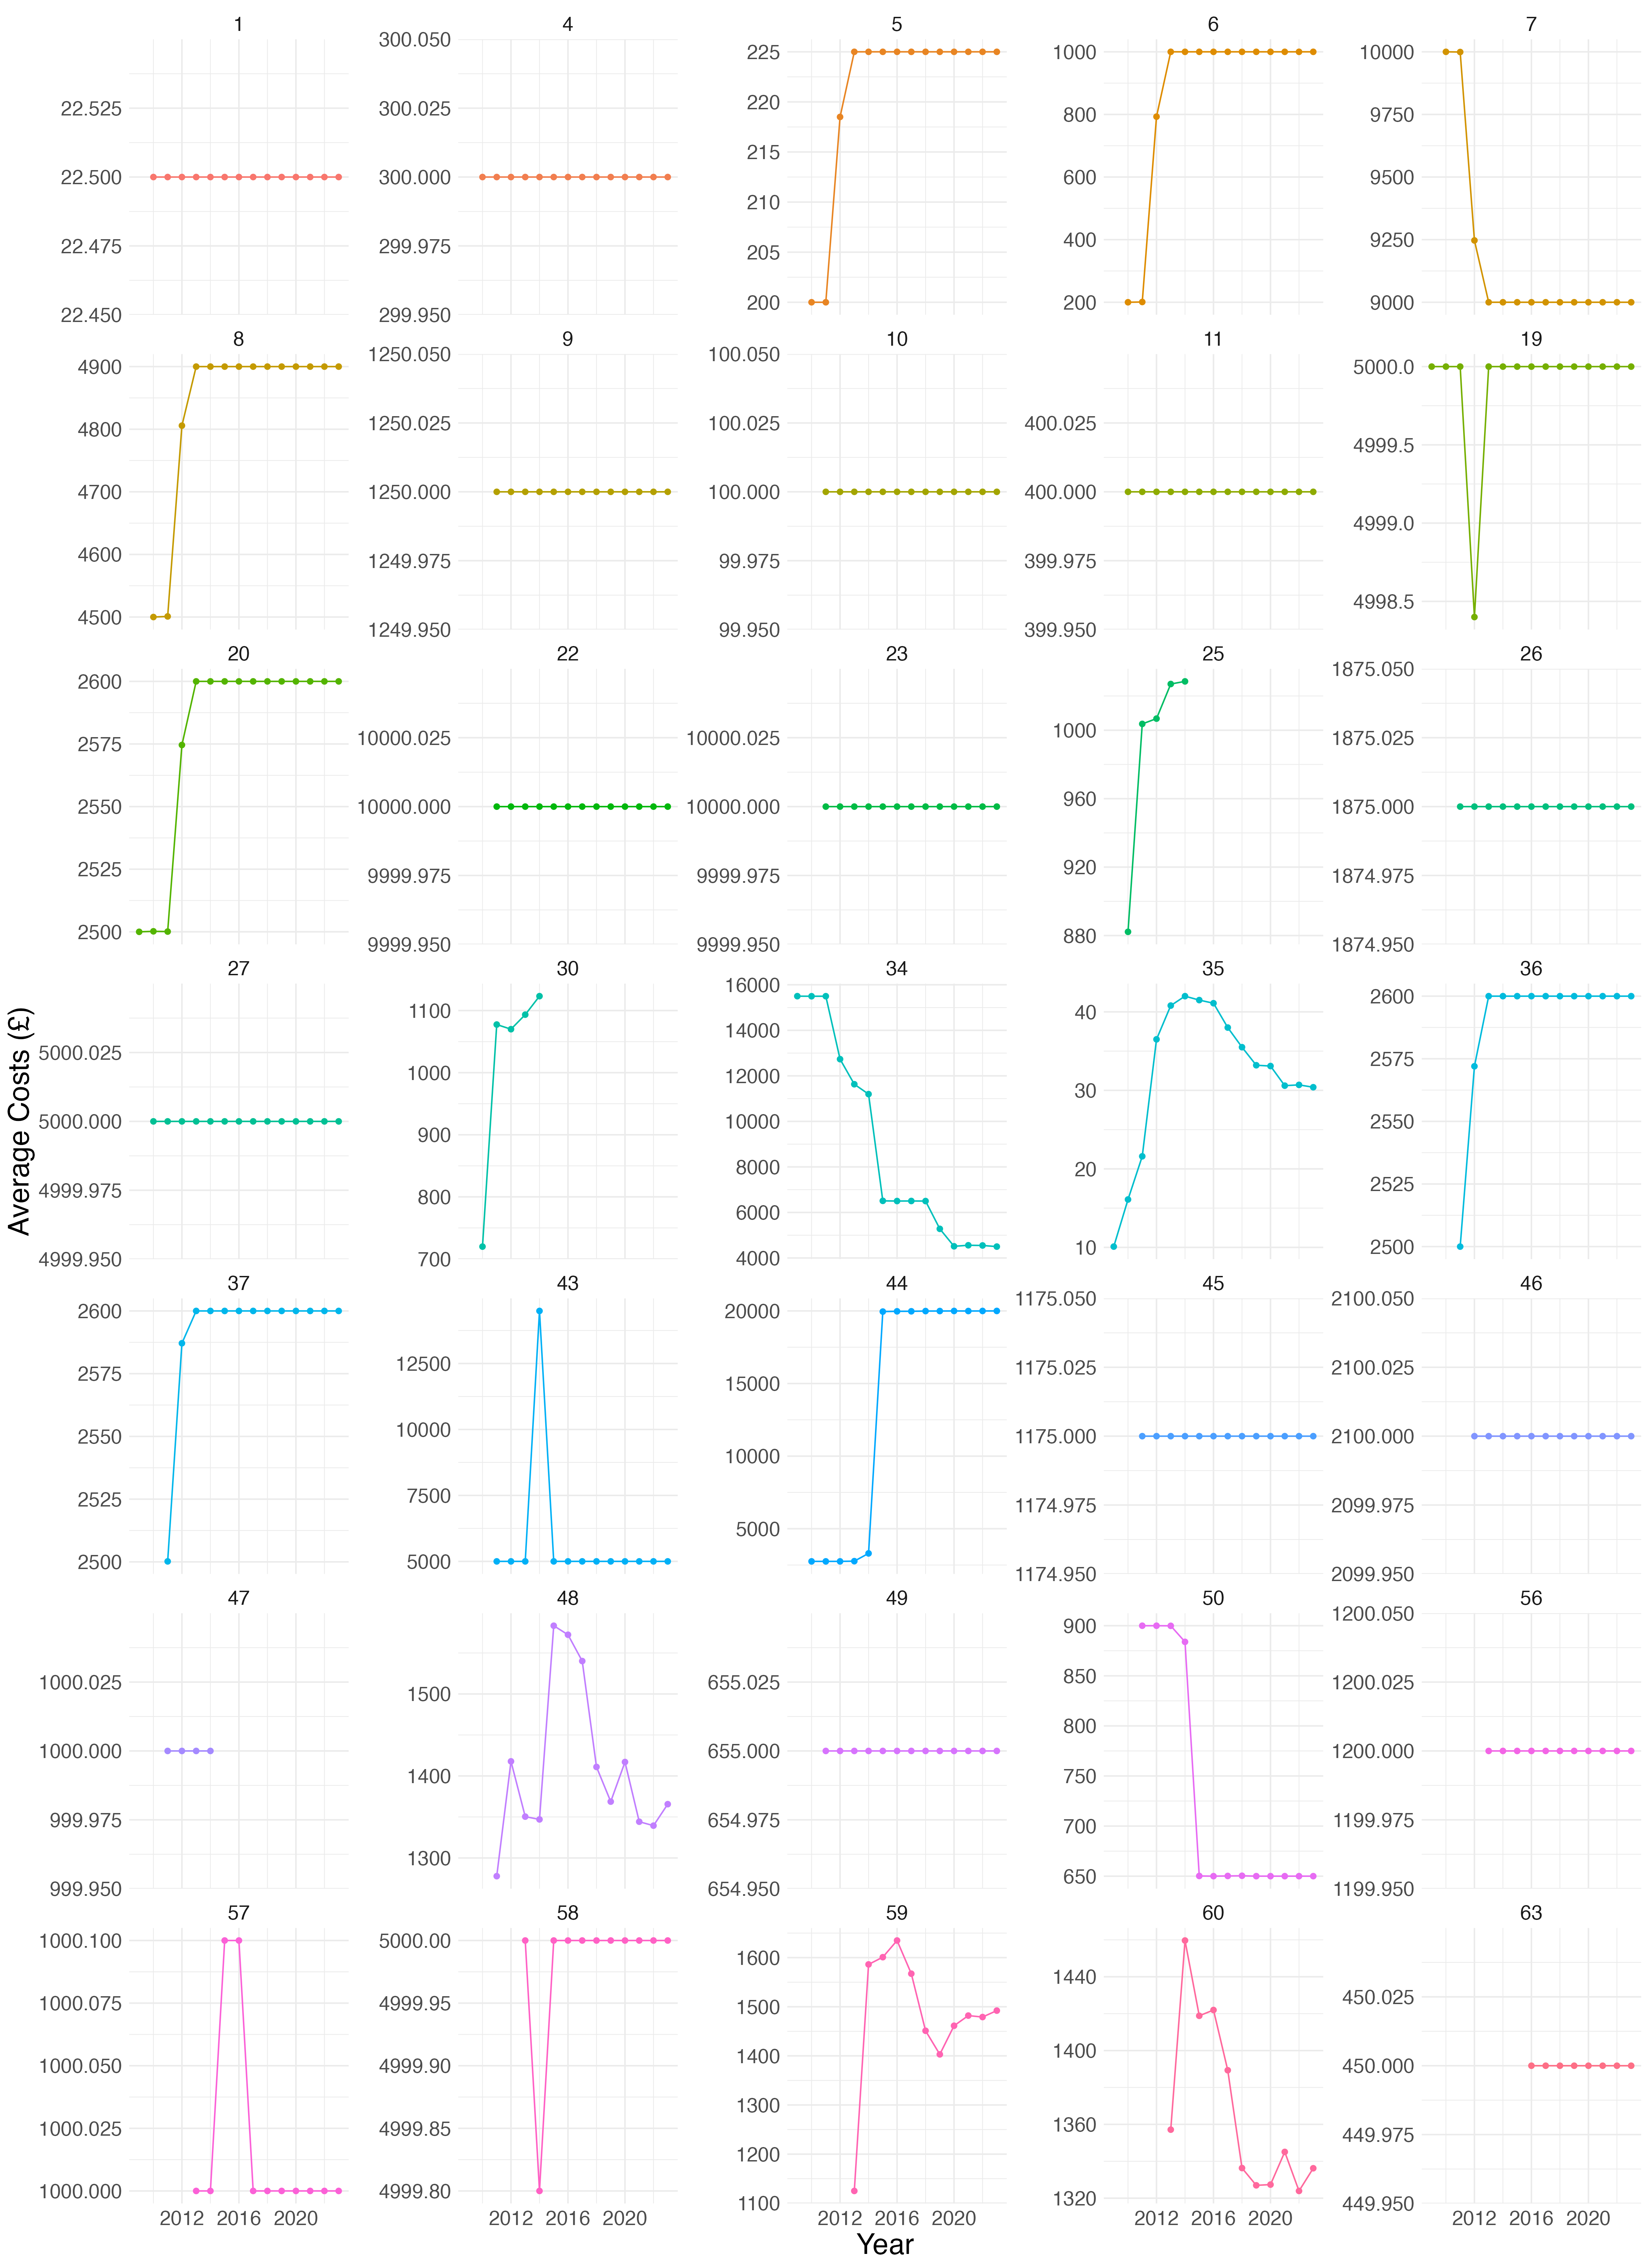
\includegraphics[width=1\textwidth]{src/figures/Facet_costs.png} % Adjust width as needed
    \caption{Average Yearly Costs by Improvement ID, extracted from EPC recommendations for all dwellings let, sold or retrofitted between 2008 - 2023}
    \label{fig:facet_price}
\end{figure}

\subsection{Price Paid Data and Listing Dataset} 
The HM Land Registry's Price Paid data provides nearly a full record of all residential property sales in England and Wales since 1995.\footnote{\textit{HM Land Registry: Price Paid Data}. (2016). [Dataset]. \href{https://www.gov.uk/government/collections/price-paid-data}{https://www.gov.uk/government/collections/price-paid-data}} Transactions excluded from the Price Paid Data are homes not registered with the HM Land Registry and all unorthodox transfer of property rights (i.e., Deeds, 'Right to Buy' discounted properties, etc.). While previously only commercially available, the UK Land Registry data became accessible to the public as of 2013, making historical records of cash and mortgage transactions open data. For the purpose for this study, variables included the transaction prices, date, location (by postcode), property type, and UPRNs. In total 14.5 million transactions were extracted from the Price Paid data between 2007-23, of which 9.6 million consisted of unique addresses (or UPRNs). \\

\begin{table}[!h]
\centering
\caption{Summary Statistics of average transaction price by property type and EPC rating as defined by RdSAP.}
\begin{tabular}{lrrrrr}
\toprule
EPC Rating & Bungalow & Flat & House & Maisonette & Park home\\
\midrule
\cellcolor{gray!10}{A} & \cellcolor{gray!10}{297144.7} & \cellcolor{gray!10}{328078.0} & \cellcolor{gray!10}{366825.9} & \cellcolor{gray!10}{384231.6} & \cellcolor{gray!10}{-}\\
B & 298159.8 & 297840.0 & 304817.2 & 342341.8 & -\\
\cellcolor{gray!10}{C} & \cellcolor{gray!10}{279565.3} & \cellcolor{gray!10}{228881.0} & \cellcolor{gray!10}{264755.1} & \cellcolor{gray!10}{254608.2} & \cellcolor{gray!10}{278219.6}\\
D & 264678.9 & 243516.0 & 264634.6 & 273549.8 & 184001.2\\
\cellcolor{gray!10}{E} & \cellcolor{gray!10}{274003.5} & \cellcolor{gray!10}{238571.2} & \cellcolor{gray!10}{283038.0} & \cellcolor{gray!10}{269317.8} & \cellcolor{gray!10}{246575.5}\\
\addlinespace
F & 277801.3 & 211757.1 & 299006.1 & 235927.6 & 226707.8\\
\cellcolor{gray!10}{G} & \cellcolor{gray!10}{256178.3} & \cellcolor{gray!10}{206546.6} & \cellcolor{gray!10}{240768.1} & \cellcolor{gray!10}{218924.4} & \cellcolor{gray!10}{291646.8}\\
\bottomrule
\label{Descriptive_Price}
\end{tabular}
\end{table}


Transaction prices were adjusted for inflation using the Retail Price Index (RPI) for the sample period which was sourced from the Office of National Statistics (ONS) \footnote{https://www.ons.gov.uk/economy/inflationandpriceindices}. While the Consumer Price Index (CPI) has been the prevailing inflation index in the UK since 2003, after its inception in 1996 \cite{office_for_national_statistics_ons_consumer_2023},  both indicators rely on the overall change in price paid by households for the goods and services they consume \cite{jonhson_uk_2015}. However, they differ in the 'basket of goods (data) and formula used \cite{levell_comparing_2012}. As seen in Figure~\ref{fig:RPIvCPI} in Appendix, the RPI relies more heavily on housing expenditures (e.g., housing purchase costs, mortgage interest payments, building insurance, etc.) making it more sensitive to housing market conditions \cite{levell_comparing_2012}. This is especially relevant during the subprime mortgage crisis, as the RPI provided a significantly better representation of the turbulent housing prices therefore, the "real" transaction prices were adjusted from the RPI as of January 2019. Properties in the top 1\% of transaction prices were considered luxury goods and hence removed from the panel of observations since they are subject to distinct consumer behaviours \cite{allsopp_additional_2005} which may directly affect the willingness to pay for certain characteristics and services such as green labels \cite{fuerst_green_2016, hui_housing_2021, fuerst_energy_2016} hence affecting the underlying trends investigated here.  \\



Finally, access to rental and sales Zoopla property data from 2016-22 were granted by Zoopla Limited\footnote{Zoopla Limited, © 2024 2. Zoopla Limited. Economic and Social Research Council. Zoopla Property Data, 2024} under licensed agreement and aggregated at postcode level each property in order to control for variations in supply in the housing market across the UK and Wales. For each property, the time period listed on the market until sold or rented was provided enabling the computation of the active listings in an area surrounding a point of transaction. For each listing period, the number of listings was therefore computing across district areas and added as controls for supply. Figure \ref{fig:active_listings} provides an overview of the supply of private homes for rent and sale as aggregated therein, as measured in the number of active listings in a given area and month, showing clear evidence of seasonal trends.

\begin{figure}[h]
    \centering
    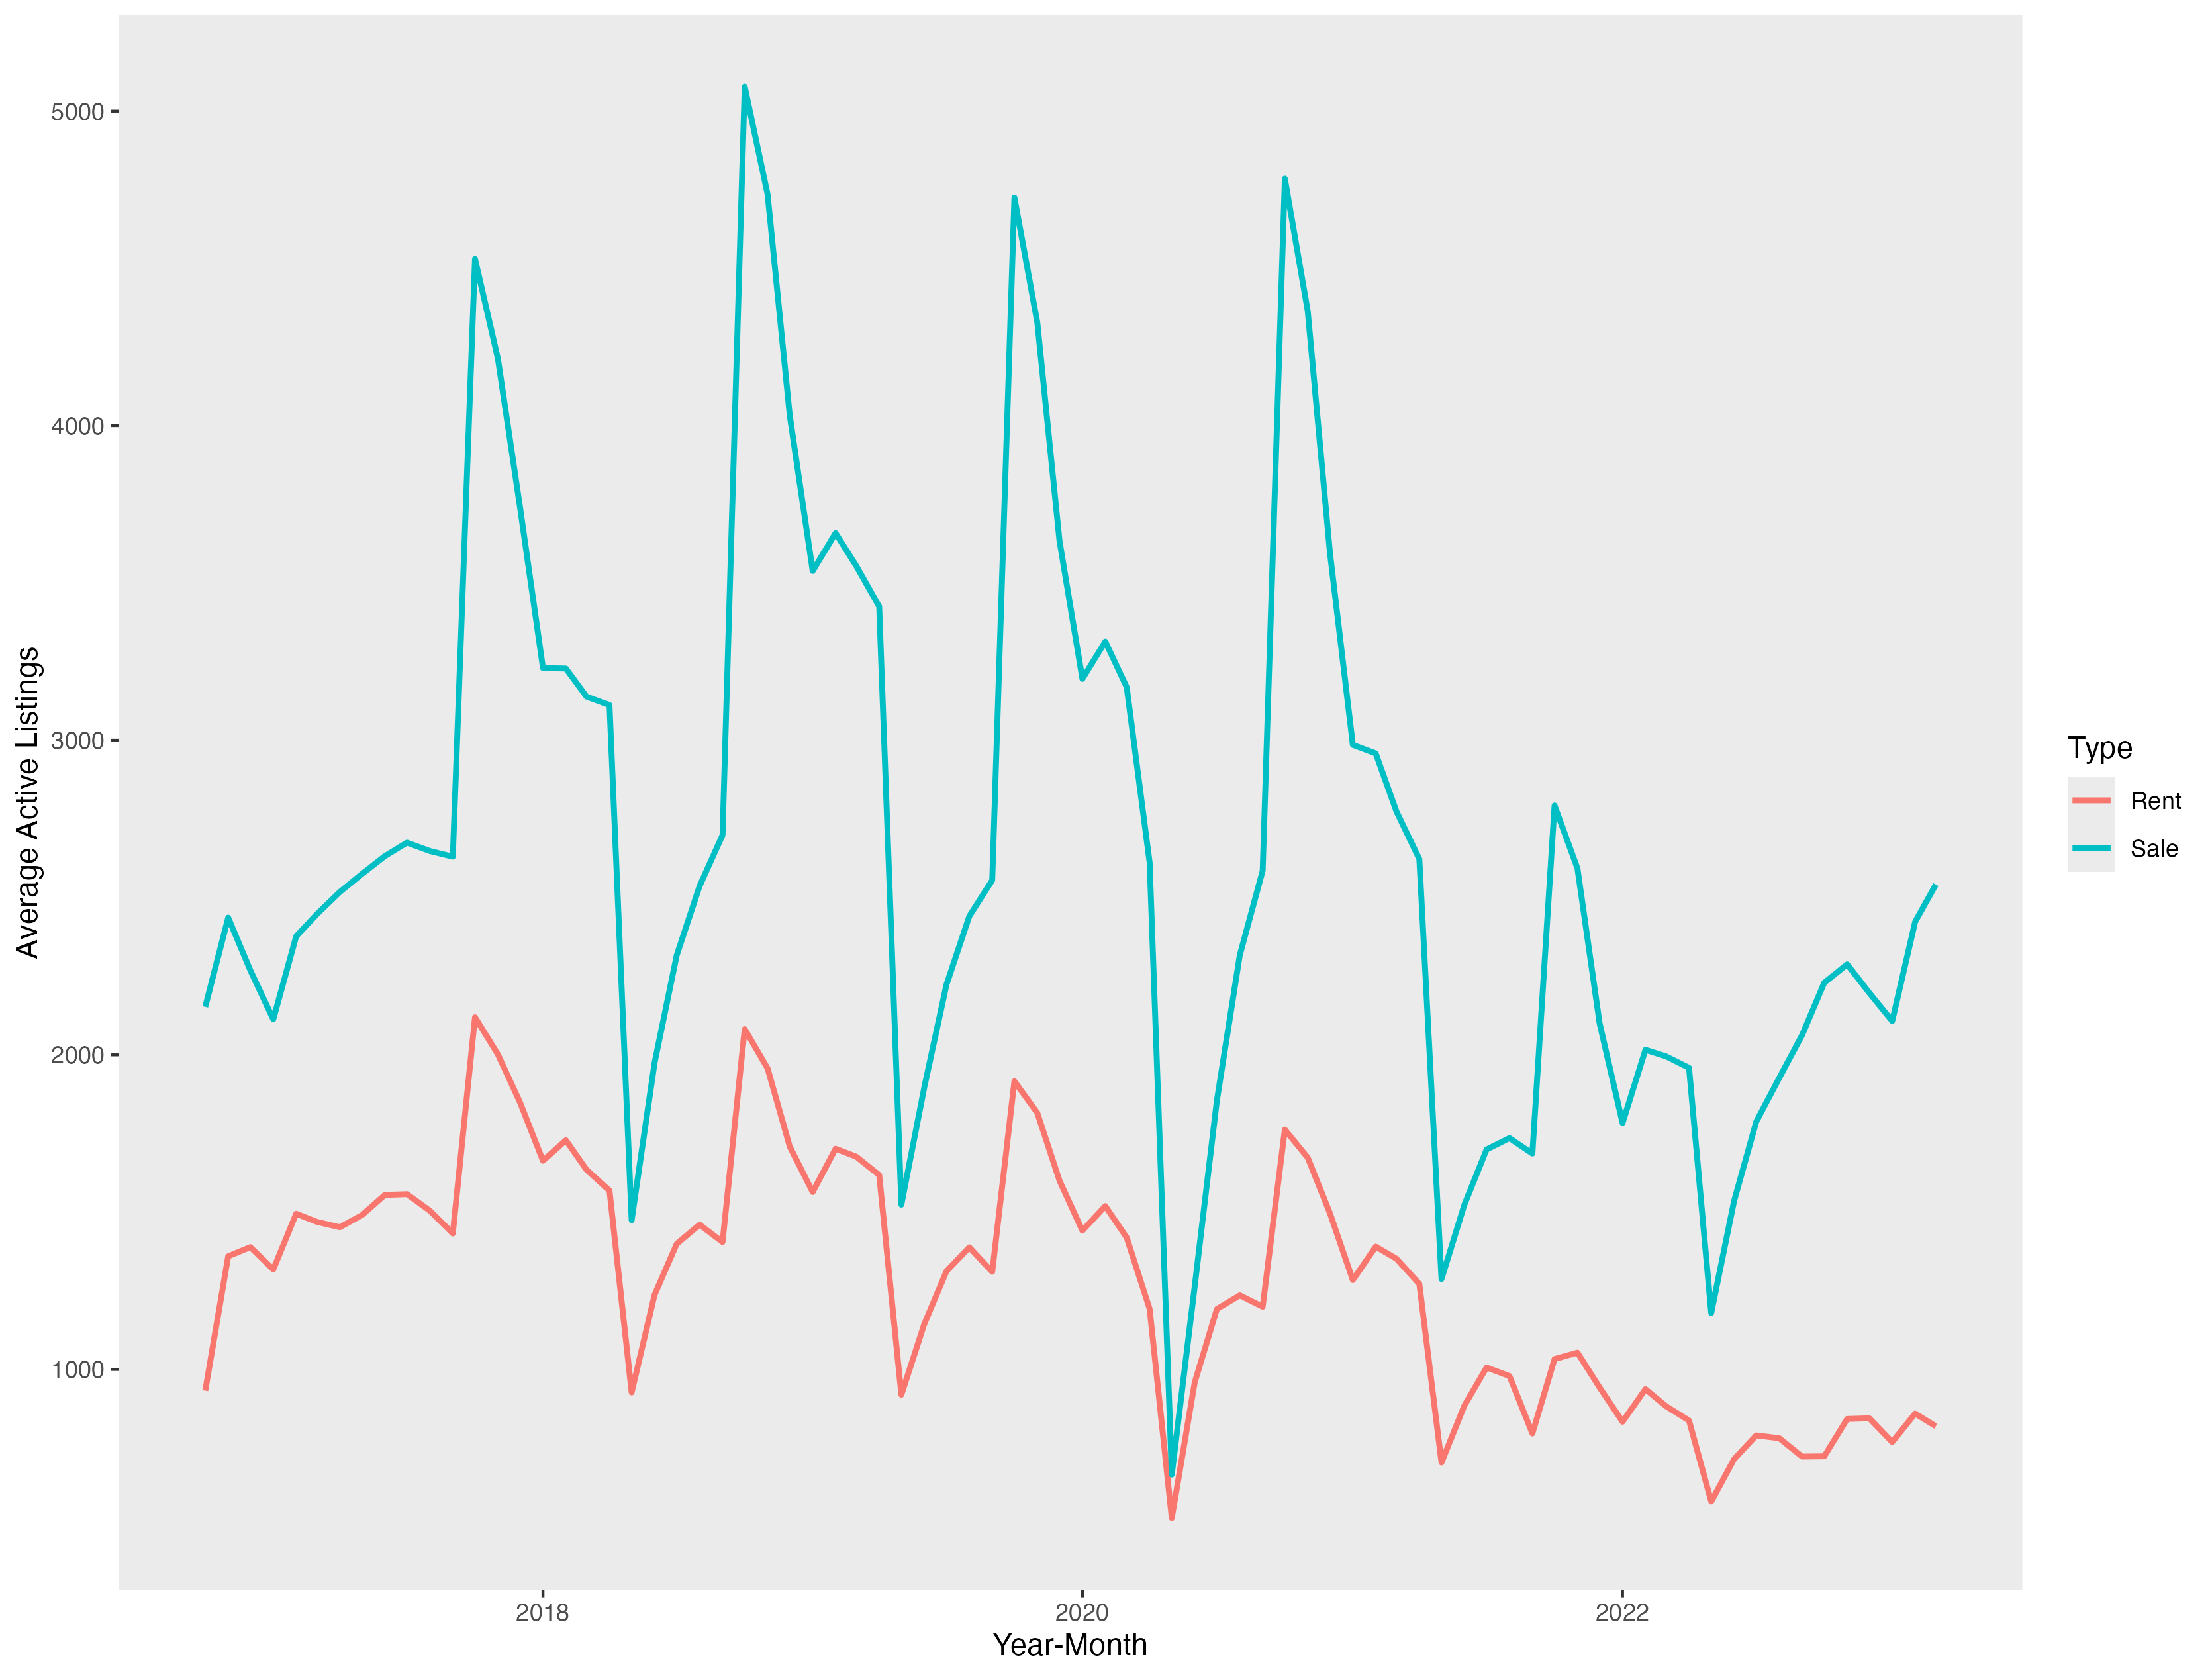
\includegraphics[width=0.75\linewidth]{src/figures/active_listings.png}
    \caption{Average monthly rental and sale active listings in UK and Wales.}
    \label{fig:active_listings}
\end{figure}




\section{Methods and Results}

In this section we explore ...

\subsection{Costing Energy Retrofits and their impacts}
Dwellings with at least one inspection recording an EPC ($15.6$ million registered), were analysed. Each EPC records current and potential energy efficiency, rating, retrofits available together with recommendation file which lists potential retrofits in a given property.

Should the property be able to raise their EPC, the record will include the potential energy rating alongside their current energy rating, respectively denoted $R_p$ and $R_c$ in the equation below, so that the difference in energy efficiency is explained by committing to specific retrofits (with $R_i$ a list of retrofits):
\begin{align*}
    E_{i,p} - E_{i,c} = f(R_{i})
\end{align*}
%In cases where the minimum or maximum costs were missing, only the given value was taken into account. For each improvement ever recommended on an EPC, each of its attributes advertised were stored, dated and averaged with its other appearances for dwelling having undergone an inspection the same year. Differences were taken across all attributes. If an improvement was no longer recommended, it was assumed it must have been implemented between inspections. This identification strategy enabled to explore a wider sample dataset than previously attempted by surveys (Coyne and Denny, 2021).\\
\noindent We start with estimating the impact of distinct energy retrofits on a series of dependent variables, including Energy Efficiency, energy consumption, costs and emissions in a given dwelling. We run the following regression using Ordinary Least Square (OLS):
\begin{align}
    Y_i = E_{i,p} -E_{i,c} = \beta_0 + \sum_{m=1}^{63} \beta_{\text{m}} X_{\text{i,m}}  + \gamma_i \cdot time_{fe} +  \epsilon_i
\label{eq:general_impacts_OLS}
\end{align}
where $Y_i$ captures Energy Efficiency (score out of 100), Yearly energy Consumption ($kWh/m^2$), costs (\textsterling  \textbackslash $kWh$) and $CO_2$ emissions. $X_{i,m}$ is a vector of energy retrofits in a given property $i$. The environmental impact ratings are based on the carbon emissions of buildings per square meter \cite{rowe_housing_2024}. Time fixed effects are captured by $time_{fe}$ and $\epsilon_i$ is the error term. \\

Results from the five OLS regressions (Eq. \ref{eq:general_impacts_OLS}) are presented in Table \ref{tab:ID_impacts} below. Coefficients are all significant (p-value less than 0.0001).  They provide insight into the marginal effects of each completed structural retrofit on the energy efficiency score, energy consumption (in kWh and £), and emissions (in CO2 and impact score) of dwellings. According to table \ref{tab:ID_impacts}, installing a wood pellet stove with boiler and radiator (ID 23 \& 39) can increase a property’s energy efficiency rating by 22.79, making this improvement option the most optimal decision when aiming to increase the EPC score ($Y_1$). As expected, improvement ID 23\&39, also yields the greatest impact with all other dependent variables, resulting in the most impact retrofit available to homeowners from a purely results-based perspective. When comparing across all the regression results, it seems the most ’impactful’ renovations involve improving a dwelling’s heating systems (e.g., Fan assisted storage heaters,
gas condensing boilers, replacing heating units, etc.). This is consistent with prior findings that the majority of residential energy consumption and associated emissions stem from space and water heating \cite{lowe_technical_2007, kesicki_costs_2012} . Conversely, the recommendations associated with the lowest impact estimates from the models, are mostly associated with fabric energy efficiency and energy conservation measures (i.e., loft insulation, double window glazing, party wall insulation, etc.). The results were appended and used during the subsequent parts of the analysis as indicators of impacts for each dwelling.  
\begin{table}[h!] 
\begin{center}
\caption{Regressions Results: Impacts of Improvements according to EPCs 2008-22}
\label{tab:ID_impacts}
\resizebox{\textwidth}{!}{ 
\begin{tabular}{r p{5cm} rrrrr | r} 
\toprule
\toprule
&   &  \multicolumn{5}{c}{\textit{Dependent Variables}}  \\
\cmidrule(lr){3-7}  % Partial midrule 
&   & \textbf{EPC(\%)} & \textbf{Consumption (kWh)} & \textbf{CO2} & \textbf{Environmental} & \textbf{Bill (\textsterling)} \\ 
 & \textit{Independent Variables} &   ($Y_1$) & ($Y_2$) & ($Y_3$) & ($Y_4$) & ($Y_5$) & \textbf{Cost (\textsterling)}\\ 
\midrule
\midrule
1-3 & Insulate hot water cylinder with 80 mm jacket & $3.66^{***}$ & $-40.56^{***}$ & $-0.37^{***}$ & $3.93^{***}$ & $-62.25^{***}$ & $22.5$ \\ 
4 & Hot water cylinder thermostat  & $4.48^{***}$ & $-32.83^{***}$ & $-0.66^{***}$ & $4.78^{***}$ & $-121.14^{***}$ & $300$\\ 
5 & Increase loft insulation to 270 mm  & $3.20^{***}$ & $-26.05^{***}$ & $-0.45^{***}$ & $3.74^{***}$ & $-93.96^{***}$ & $225$\\ 
6 & Cavity wall insulation  & $4.79^{***}$ & $-40.68^{***}$ & $-0.64^{***}$ & $5.48^{***}$ & $-126.39^{***}$ & $1000$\\ 
7 & 50 mm internal or external wall insulation & $6.30^{***}$ & $-52.08^{***}$ & $-0.89^{***}$ & $7.01^{***}$ & $-186.02^{***}$ & $9000$\\ 
8 & Replace single glazed windows with low-E double glazing  & $2.31^{***}$ & $-21.55^{***}$ & $-0.45^{***}$ & $2.22^{***}$ & $-90.07^{***}$ & $4900$\\ 
9 & Secondary glazing to single glazed windows & $2.44^{***}$ & $-12.72^{***}$ & $-0.66^{***}$ & $1.26^{***}$ & $-110.11^{***}$ & $1250$\\ 
10 & Draughtproof single-glazed windows  & $4.46^{***}$ & $-28.88^{***}$ & $-1.01^{***}$ & $3.99^{***}$ & $-198.74^{***}$ & $100$\\ 
11-18 & Upgrade heating controls  & $2.29^{***}$ & $-15.11^{***}$ & $-0.32^{***}$ & $2.60^{***}$ & $-62.79^{***}$ & $400$ \\ 
19 & Solar water heating  & $2.84^{***}$ & $-30.54^{***}$ & $0.47^{***}$ & $3.20^{***}$ & $84.64^{***}$ & $5000$\\ 
20-21 & Replace boiler with new condensing boiler  & $4.39^{***}$ & $-33.06^{***}$ & $-0.75^{***}$ & $5.53^{***}$ & $-139.94^{***}$ & $2550$\\ 
22 & Replace boiler with biomass boiler  & $14.62^{***}$ & $-106.26^{***}$ & $-11.78^{***}$ & $57.12^{***}$ & $-585.71^{***}$ & $10000$\\ 
23\&39 & Wood pellet stove with boiler and radiators  & $22.79^{***}$ & $-234.00^{***}$ & $-14.62^{***}$ & $58.98^{***}$ & $-1161.85^{***}$ & $10000$\\ 
24\&30 & Fan assisted storage heaters and Dual Immersion Cylinder & $9.19^{***}$ & $-58.68^{***}$ & $-0.75^{***}$ & $4.89^{***}$ & $-179.76^{***}$ & $1123.8$\\ 
25\&31 & Fan-assisted storage heaters & $9.19^{***}$ & $-58.68^{***}$ & $-0.75^{***}$ & $4.89^{***}$ & $-179.76^{***}$ & $998.75$\\ 
26 & Replacement warm air unit & $2.38^{***}$ & $-14.73^{***}$ & $-0.38^{***}$ & $3.00^{***}$ & $-95.81^{***}$ & $1875$\\ 
27,29,32,40-42 & Change heating to gas condensing boiler & $18.36^{***}$ & $-173.60^{***}$ & $-2.20^{***}$ & $17.87^{***}$ & $-586.96^{***}$ & $5000$\\ 
28\&43 & Condensing oil boiler with radiators & $10.24^{***}$ & $-18.21^{***}$ & $-2.72^{***}$ & $7.53^{***}$ & $-429.72^{***}$ & $12500$\\ 
34 & Solar photovoltaic panels, 2.5 kWp  & $6.41^{***}$ & $-27.92^{***}$ & $-1.47^{***}$ & $5.01^{***}$ & $-145.52^{***}$ & $4500$\\ 
35 & Low energy lighting for all fixed outlets  & $0.88^{***}$ & $-5.38^{***}$ & $-0.11^{***}$ & $0.82^{***}$ & $-35.12^{***}$ & $30.40$\\ 
36 & Replace heating unit with condensing unit  & $2.92^{***}$ & $-22.77^{***}$ & $-0.40^{***}$ & $3.50^{***}$ & $-83.92^{***}$ & $2600$ \\ 
37-38 & Install condensing boiler  & $13.65^{***}$ & $-47.16^{***}$ & $-3.99^{***}$ & $11.48^{***}$ & $-680.93^{***}$ & $2600$\\ 
44 & Wind turbine & $6.20^{***}$ & $-37.59^{***}$ & $-0.87^{***}$ & $4.66^{***}$ & $-70.00^{***}$ & $19999.3$\\ 
45 & Flat roof insulation  & $4.05^{***}$ & $-35.29^{***}$ & $-0.60^{***}$ & $4.49^{***}$ & $-132.82^{***}$ & $1175$\\ 
46 & Room-in-roof insulation & $7.57^{***}$ & $-49.07^{***}$ & $-1.92^{***}$ & $8.32^{***}$ & $-398.64^{***}$ & $2100$\\ 
47 & Floor insulation & $5.41^{***}$ & $-33.05^{***}$ & $-0.63^{***}$ & $6.38^{***}$ & $-88.26^{***}$ & $1000$\\ 
48 & High performance external doors & $5.07^{***}$ & $-50.21^{***}$ & $-0.22^{***}$ & $3.50^{***}$ & $-77.32^{***}$ & $1365.6$ \\ 
49 & Heat recovery system for mixer showers & $1.49^{***}$ & $-50.21^{***}$ & $-0.09^{***}$ & $1.01^{***}$ & $-50.43^{***}$ & $655$\\ 
50 & Flue gas heat recovery device in conjunction with boiler & $3.81^{***}$ & $-42.05^{***}$ & $0.56^{***}$ & $2.85^{***}$ & $80.30^{***}$ & $650$\\ 
56 & Replacement glazing units  & $1.49^{***}$ & $-16.67^{***}$ & $-0.15^{***}$ & $2.24^{***}$ & $-29.63^{***}$ & $1200$\\ 
57 & Suspended floor insulation  & $4.01^{***}$ & $-32.61^{***}$ & $-0.58^{***}$ & $4.65^{***}$ & $-114.17^{***}$ & $1000$\\ 
58 & Solid floor insulation & $4.44^{***}$ & $-34.68^{***}$ & $-0.64^{***}$ & $4.62^{***}$ & $-112.41^{***}$ & $5000$\\ 
59\&61 & High heat retention storage heaters and dual immersion cylinder & $17.32^{***}$ & $-85.81^{***}$ & $-0.72^{***}$ & $4.21^{***}$ & $-489.40^{***}$ & $1501.3$\\ 
60\&62 & High heat retention storage heaters & $9.14^{***}$ & $-64.51^{***}$ & $-0.49^{***}$ & $3.55^{***}$ & $-249.02^{***}$ & $1346.1$\\ 
63 & Party wall insulation & $2.53^{***}$ & $-32.71^{***}$ & $-0.14^{***}$ & $3.30^{***}$ & $-24.36^{***}$ & $450$\\
\addlinespace
\midrule
& Year Fixed.E     & \textit{yes}    & \textit{yes}  & \textit{yes} & \textit{yes} & \textit{yes} \\
& Efficiency Gradings    & \textit{yes}    & \textit{yes}  & \textit{yes} & \textit{yes} & \textit{yes} \\
\bottomrule
\bottomrule
\end{tabular}
}
\end{center}
\caption*{\scriptsize{\textit{\small{\textbf{NOTES:} These estimates are the results of OLS regressions. The table reports the impacts of each improvement (independent variables). The coefficients represent the change in the dependent variables per improvement completed (independent variable). The columns report the estimated impact of each improvement on the change in EPC($Y_1$), change in Energy Consumption($Y_2$), $CO_2$ emissions ($Y_3$), Environmental Impact factor ($Y_4$), and total energy costs in ($Y_5$). Regressions include household fixed effects, along with time controls in the second column. Robust standard errors in parentheses. Significance levels are indicated as $^{***}p<0.001$; $^{**}p<0.01$; $^{*}p<0.05$}}}}

\end{table}


\subsection{Cumulative costs and environmental impacts of reaching EPC-C}

As previously mentioned, property owners are not obligated but highly encouraged to follow the ordered improvement suggestions on the EPC \cite{department_for_communities_and_local_government_guide_2017}. Figure \ref{fig:decision_models} provides an overview of the 3 'retrofitting strategies' used to model the complex decision-making process of property owners willing to retrofit. Faced with the EPC recommendations lists, owners can opt for the 'low hanging fruit' improvements if faced with requirements to retrofit and low financial capabilities \cite{jones_retrofitting_2013}. In this strategy, it is assumed the cheapest structural retrofitting suggestions would be firstly implemented. Conversely, the strategy 4 would highlight dwellings willing to invest first in improvements that could yield the highest impact (change in EPC score) to retrofit with minimal interventions. Finally, a more complex scenario is explored (strategy 3). In this model, it is assumed homeowners could estimate the 'highest impact per pound' improvements and preferably selected such impactful and worth-while retrofits. \\

\begin{figure}[h!]
    \centering
    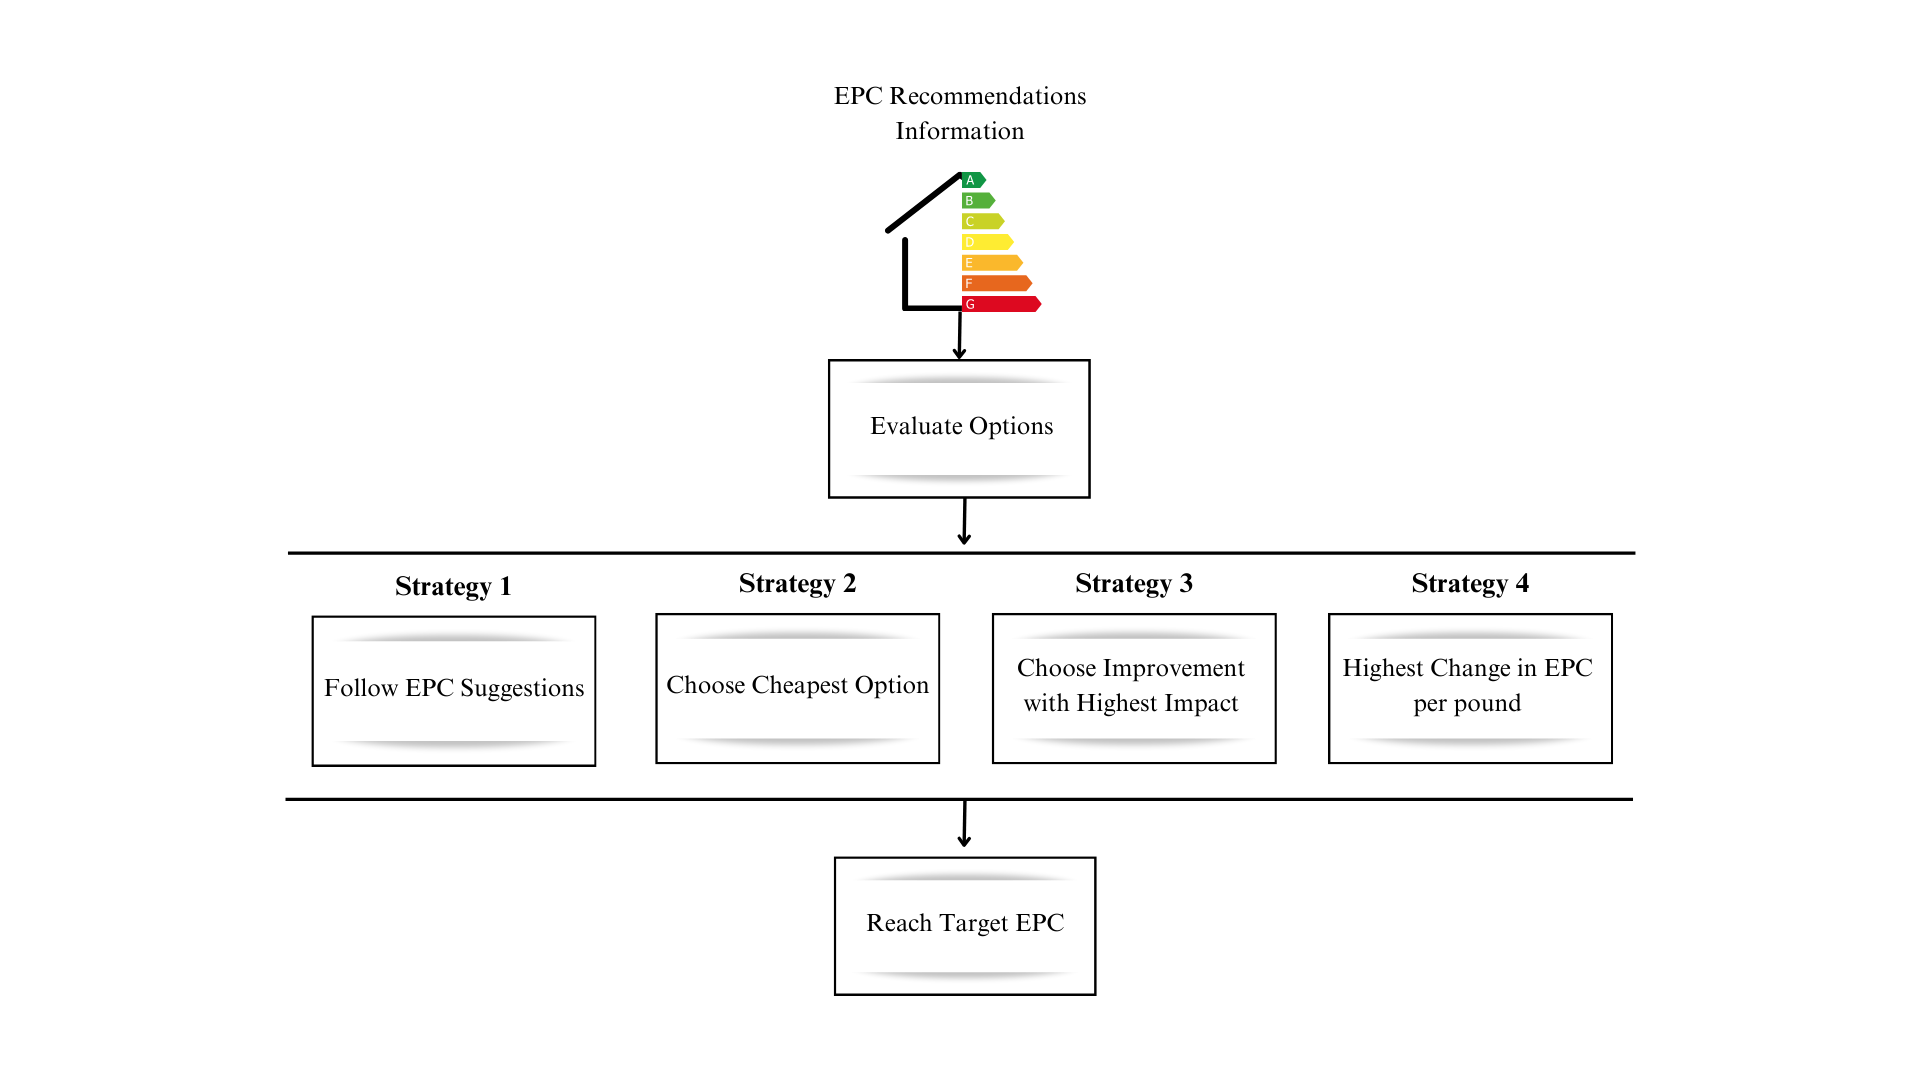
\includegraphics[width=1\linewidth]{src/figures/decision_model.png}
    \caption{Conceptual framework of decision models used to estimate cost of reaching minimum energy efficiency. The strategies were executed as separate rule-based algorithms applied to the latest energy performance certificates for every unique properties.}
    \label{fig:decision_models}
\end{figure}


The cumulative costs of achieving the EPC cap was determined for each nuanced retrofitting strategy: 1) per EPC recommendation, 2) as per EPC impact potential, 3) cheapest improvement option) and 4) by best impact per investment (EPC\_impact/Cost of retrofit). The program ran on the $9.2$ million dwellings that were able to rise their EPCs and had an original energy efficiency below that of the MEES amendment suggested of $69\%$ (C-Band).  The linear estimation models overestimated the cumulative and individual costs and impacts of reaching the minimum EPC rating standards (Table \ref{EPC_69_costs}). This was probably induced as the linear estimation included some costly improvements at the of the EPC recommendations which would have yielded more than the necessary scores. Conversely, the computationally-determined costs using different 'strategies' stopped keeping track of structural improvements once households reached the set threshold. The total costs for retrofitting all able registered properties in England and Wales to an EPC rating of C range from \textsterling 59 billion to \textsterling 94 billion, allowing the sector to reduce its yearly emissions by 18.1 - 20 million tonnes of $CO_2{eq}$. In 2023, residential emissions from buildings in the UK accounted for 51.7 million tones of $CO_2{eq}$ \footnote{2023 Provisional figures from ONS and DESNZ}. The cumulative costs would be estimated at about \textsterling 82.5 billion if all home owners followed and implemented the list of recommendations provided by their EPCs. For each investment strategy, the cumulative change in energy consumption for the housing sector is also displayed and presented in $GWh/m^2$. While the EPC retrofitting strategy does not yield the greatest decrease in emissions, SAP recommendations allow for the most significant decrease in energy consumption. \\

% Include the table on total costs
% add ordered by carbon reduction, remove ENv column
\begin{table}[!h]
\caption{Cumulative Costs for EPC Cap 69}
\label{EPC_69_costs}
\centering
\resizebox{\ifdim\width>\linewidth\linewidth\else\width\fi}{!}{
\begin{tabular}[t]{lrlrrrr}
\toprule
\toprule
 & \textbf{N. Retrofits} & \textbf{Household} (\textsterling) & \textbf{CO2 ($MtCO_eq/yr$)} & \textbf{Env}($MtCO_eq/yr$)  & \textbf{Energy ($GWh/m^2$)} & \textbf{Total Cost} (\textsterling)\\

\midrule

\cellcolor{gray!10}{By Yield}  & \cellcolor{gray!10}{3} & \cellcolor{gray!10}{6597} & \cellcolor{gray!10}{-18.6} & \cellcolor{gray!10}{124.4} & \cellcolor{gray!10}{-881.6} & \cellcolor{gray!10}{60,887,982,229}\\

By Price & 3 & 6670 & -18.3 & 124.6 & -885.2 & 61,558,192,060\\

\cellcolor{gray!10}{By EPC} & \cellcolor{gray!10}{3} & \cellcolor{gray!10}{9058} & \cellcolor{gray!10}{-16.1} & \cellcolor{gray!10}{125.3} & \cellcolor{gray!10}{-918.3} & \cellcolor{gray!10}{83,179,781,006}\\

Linear Est.  & - & 9705 & -12.8 & 103.6 & -739.1 & 89,649,163,609 \\

\cellcolor{gray!10}{By Impact} & \cellcolor{gray!10}{2} & \cellcolor{gray!10}{9820} & \cellcolor{gray!10}{-20.6} & \cellcolor{gray!10}{115.5} & \cellcolor{gray!10}{-806.5} & \cellcolor{gray!10}{90,633,857,958}\\
\bottomrule
\end{tabular}}
\caption*{\small \textit{\textbf{NOTES:} Results were determined by accumulating retrofitting costs for all houses in need and capable of reaching an energy performance score of 69. The rule-based program ran on 9.2 million dwellings, following the EPC Recommendations (Strategy \#1 in Figure \ref{fig:decision_models}).}}


\end{table}


According to the table therein, the “cheapest” aggregate option to reach an EPC of 69 is achieved when property owners opt in for the improvement that can yield the highest impact on energy efficiency for the lowest price. This option would require significant investments in Solar Photovoltaic Panels (nearly 4 million across the UK) and over £13 billion national investments for external wall insulations (see table \ref{costs_yield}). Following this decision mode, reaching an EPC of 69 would require households to spend £6597 on retrofitting costs on average which would present significant savings when compared to the order recommended by the EPC assessments. Indeed, to achieve an EPC of 69 following the SAP recommendations, the average household would have to spend nearly £9000 on retrofitting costs, most of which would require investment in PV panels and solar water heating. See Appendix \ref{sec:appendix} for other improvement strategies. This confirms \cite{billio_learning_2024} study which suggested applying more complex and sophisticated methods of selecting structural improvements result in cheaper and more efficient outcomes. While the low-hanging fruit strategies (by yield or by price) provide the most cost-effective means of achieving MEES, they do not effectively reduce $CO_2$ emissions as much as strategies focused on impact.  Similarly, following the EPC recommendations result in less emission reductions but yield the highest reduction in energy consumption (expressed in GWh per area in Table \ref{EPC_69_costs}). These observations confirm \cite{kelly_building_2012} suggestions that the SAP methodologies and recommendations may create perverse incentives to reduce energy consumption rather than limit environmental damages. \\
 \begin{table}[!h]
\centering
\caption{Total Needed Improvements to Reach EPC C ordered by Total Costs, according to 'Highest Yield' decision strategy.}
\centering
\resizebox{\ifdim\width>\linewidth\linewidth\else\width\fi}{!}{
\begin{tabular}[t]{cc p{7cm} ccccc}
\toprule
ID & Count & Description & COST (\textsterling) & $\Delta$EPC & Energy($KWh$) & CO2 ($CO_2{eq}/yr$) & TOTAL COSTS (\textsterling)\\
\midrule
\cellcolor{gray!10}{34} & \cellcolor{gray!10}{3922456} & \cellcolor{gray!10}{Solar photovoltaic panels, 2.5 kWp} & \cellcolor{gray!10}{4500} & \cellcolor{gray!10}{6} & \cellcolor{gray!10}{-1.469} & \cellcolor{gray!10}{-27.922} & \cellcolor{gray!10}{17651052000}\\
7 & 1449750 & 50 mm internal or external wall insulation & 9000 & 6 & -0.886 & -52.080 & 13047750000\\
\cellcolor{gray!10}{20} & \cellcolor{gray!10}{2247525} & \cellcolor{gray!10}{Replace boiler with new condensing boiler} & \cellcolor{gray!10}{2550} & \cellcolor{gray!10}{4} & \cellcolor{gray!10}{-0.752} & \cellcolor{gray!10}{-33.063} & \cellcolor{gray!10}{5731301126}\\
58 & 833332 & Solid floor insulation & 5000 & 4 & -0.636 & -34.684 & 4166660000\\
\cellcolor{gray!10}{19} & \cellcolor{gray!10}{801603} & \cellcolor{gray!10}{Solar water heating} & \cellcolor{gray!10}{5000} & \cellcolor{gray!10}{3} & \cellcolor{gray!10}{0.474} & \cellcolor{gray!10}{-30.535} & \cellcolor{gray!10}{4008015000}\\
\addlinespace
44 & 156729 & Wind turbine & 19999 & 6 & -0.870 & -37.588 & 3134470290\\
\cellcolor{gray!10}{6} & \cellcolor{gray!10}{2133786} & \cellcolor{gray!10}{Cavity wall insulation} & \cellcolor{gray!10}{1000} & \cellcolor{gray!10}{5} & \cellcolor{gray!10}{-0.641} & \cellcolor{gray!10}{-40.683} & \cellcolor{gray!10}{2133786000}\\
57 & 1851908 & Suspended floor insulation & 1000 & 4 & -0.583 & -32.612 & 1851908000\\
\cellcolor{gray!10}{47} & \cellcolor{gray!10}{1565764} & \cellcolor{gray!10}{Floor insulation} & \cellcolor{gray!10}{1000} & \cellcolor{gray!10}{5} & \cellcolor{gray!10}{-0.630} & \cellcolor{gray!10}{-33.051} & \cellcolor{gray!10}{1565764000}\\
8 & 262302 & Replace single glazed windows with low-E double glazing & 4900 & 2 & -0.451 & -21.554 & 1285279800\\
\addlinespace
\cellcolor{gray!10}{11} & \cellcolor{gray!10}{2874681} & \cellcolor{gray!10}{Upgrade heating controls} & \cellcolor{gray!10}{400} & \cellcolor{gray!10}{2} & \cellcolor{gray!10}{-0.319} & \cellcolor{gray!10}{-15.115} & \cellcolor{gray!10}{1149872400}\\
46 & 498424 & Room-in-roof insulation & 2100 & 8 & -1.919 & -49.068 & 1046690400\\
\cellcolor{gray!10}{27} & \cellcolor{gray!10}{201053} & \cellcolor{gray!10}{Change heating to gas condensing boiler} & \cellcolor{gray!10}{5000} & \cellcolor{gray!10}{18} & \cellcolor{gray!10}{-2.203} & \cellcolor{gray!10}{-173.602} & \cellcolor{gray!10}{1005265000}\\
45 & 463028 & Flat roof insulation & 1175 & 4 & -0.604 & -35.291 & 544057900\\
\cellcolor{gray!10}{5} & \cellcolor{gray!10}{1850553} & \cellcolor{gray!10}{Increase loft insulation to 270 mm} & \cellcolor{gray!10}{225} & \cellcolor{gray!10}{3} & \cellcolor{gray!10}{-0.452} & \cellcolor{gray!10}{-26.047} & \cellcolor{gray!10}{416374425}\\
\addlinespace
59 & 255465 & High heat retention storage heaters and dual immersion cylinder & 1501 & 17 & -0.724 & -85.813 & 383529604\\
\cellcolor{gray!10}{60} & \cellcolor{gray!10}{254942} & \cellcolor{gray!10}{High heat retention storage heaters} & \cellcolor{gray!10}{1346} & \cellcolor{gray!10}{9} & \cellcolor{gray!10}{-0.489} & \cellcolor{gray!10}{-64.509} & \cellcolor{gray!10}{343177426}\\
48 & 169938 & High performance external doors & 1366 & 5 & -0.215 & -50.209 & 232067333\\
\cellcolor{gray!10}{50} & \cellcolor{gray!10}{276928} & \cellcolor{gray!10}{Flue gas heat recovery device in conjunction with boiler} & \cellcolor{gray!10}{650} & \cellcolor{gray!10}{4} & \cellcolor{gray!10}{0.562} & \cellcolor{gray!10}{-42.050} & \cellcolor{gray!10}{180003200}\\
35 & 5658145 & Low energy lighting for all fixed outlets & 30 & 1 & -0.108 & -5.385 & 172007608\\
\addlinespace
\cellcolor{gray!10}{4} & \cellcolor{gray!10}{559005} & \cellcolor{gray!10}{Hot water cylinder thermostat} & \cellcolor{gray!10}{300} & \cellcolor{gray!10}{4} & \cellcolor{gray!10}{-0.663} & \cellcolor{gray!10}{-32.833} & \cellcolor{gray!10}{167701500}\\
56 & 88441 & Replacement glazing units & 1200 & 1 & -0.146 & -16.667 & 106129200\\
\cellcolor{gray!10}{30} & \cellcolor{gray!10}{85158} & \cellcolor{gray!10}{Fan assisted storage heaters and dual immersion cylinder} & \cellcolor{gray!10}{1124} & \cellcolor{gray!10}{16} & \cellcolor{gray!10}{-0.754} & \cellcolor{gray!10}{-67.301} & \cellcolor{gray!10}{95700560}\\
23 & 7706 & Wood pellet stove with boiler and radiators & 10000 & 23 & -14.619 & -235.002 & 77060000\\
\cellcolor{gray!10}{25} & \cellcolor{gray!10}{75892} & \cellcolor{gray!10}{Fan assisted storage heaters} & \cellcolor{gray!10}{999} & \cellcolor{gray!10}{9} & \cellcolor{gray!10}{-0.751} & \cellcolor{gray!10}{-58.682} & \cellcolor{gray!10}{75797135}\\
\addlinespace
10 & 620982 & Draughtproof single-glazed windows & 100 & 4 & -1.012 & -28.884 & 62098200\\
\cellcolor{gray!10}{37} & \cellcolor{gray!10}{19747} & \cellcolor{gray!10}{Install condensing boiler} & \cellcolor{gray!10}{2600} & \cellcolor{gray!10}{14} & \cellcolor{gray!10}{-3.988} & \cellcolor{gray!10}{-47.163} & \cellcolor{gray!10}{51342200}\\
63 & 109772 & Party wall insulation & 450 & 3 & -0.142 & -32.712 & 49397400\\
\cellcolor{gray!10}{49} & \cellcolor{gray!10}{67828} & \cellcolor{gray!10}{Heat recovery system for mixer showers} & \cellcolor{gray!10}{655} & \cellcolor{gray!10}{1} & \cellcolor{gray!10}{-0.089} & \cellcolor{gray!10}{-7.041} & \cellcolor{gray!10}{44427340}\\
26 & 16886 & Replacement warm air unit & 1875 & 2 & -0.380 & -14.726 & 31661250\\
\addlinespace
\cellcolor{gray!10}{22} & \cellcolor{gray!10}{2870} & \cellcolor{gray!10}{Replace boiler with biomass boiler} & \cellcolor{gray!10}{10000} & \cellcolor{gray!10}{15} & \cellcolor{gray!10}{-11.784} & \cellcolor{gray!10}{-106.260} & \cellcolor{gray!10}{28700000}\\
1 & 1148041 & Insulate hot water cylinder with 80 mm jacket & 22 & 4 & -0.366 & -40.557 & 25830922\\
\cellcolor{gray!10}{9} & \cellcolor{gray!10}{10160} & \cellcolor{gray!10}{Secondary glazing to single glazed windows} & \cellcolor{gray!10}{1250} & \cellcolor{gray!10}{2} & \cellcolor{gray!10}{-0.661} & \cellcolor{gray!10}{-12.716} & \cellcolor{gray!10}{12700000}\\
43 & 744 & Condensing oil boiler with radiators & 12500 & 10 & -2.715 & -18.210 & 9300000\\
\cellcolor{gray!10}{36} & \cellcolor{gray!10}{425} & \cellcolor{gray!10}{Replace heating unit with condensing unit} & \cellcolor{gray!10}{2600} & \cellcolor{gray!10}{3} & \cellcolor{gray!10}{-0.396} & \cellcolor{gray!10}{-22.771} & \cellcolor{gray!10}{1105000}\\
\bottomrule
\end{tabular}}
\end{table}
 
While the average reported costs for the each retrofitting strategies are specified in table \ref{EPC_69_costs}, the uni-dimensional values do not capture the heterogeneous costs across difference properties. The density plot (Figure \ref{fig:density_plot}) reveals the variation of house price around the mean reported cost following the EPC recommendations (red-dashed line).  The multi-modal distribution of retrofitting costs seem to suggest costs are grouped into multiple price ranges - potentially indicating groups of similar property characteristics. Retrofitting costs seem to be similar across price ranges. The majority of homes likely require low retrofitting costs while the long-tail suggests certain outliers require expensive investments to achieve the minimum energy efficiency standards - most of which seem to be higher priced homes (500k+). These tails persisted despite excluding the top 1\% most expensive properties to retrofitting. Out of nearly $4.45 $ million dwellings analysed, $60.95\%$ of those able to reach a minimum EPC score of 69 endure retrofitting costs less than \textsterling $ 10,000$  to retrofit, while only  $28.39\%$ fall below \textsterling  $3,500$ - according to the EPC retrofitting strategy.  \\
\begin{figure}[h!]
    \centering
    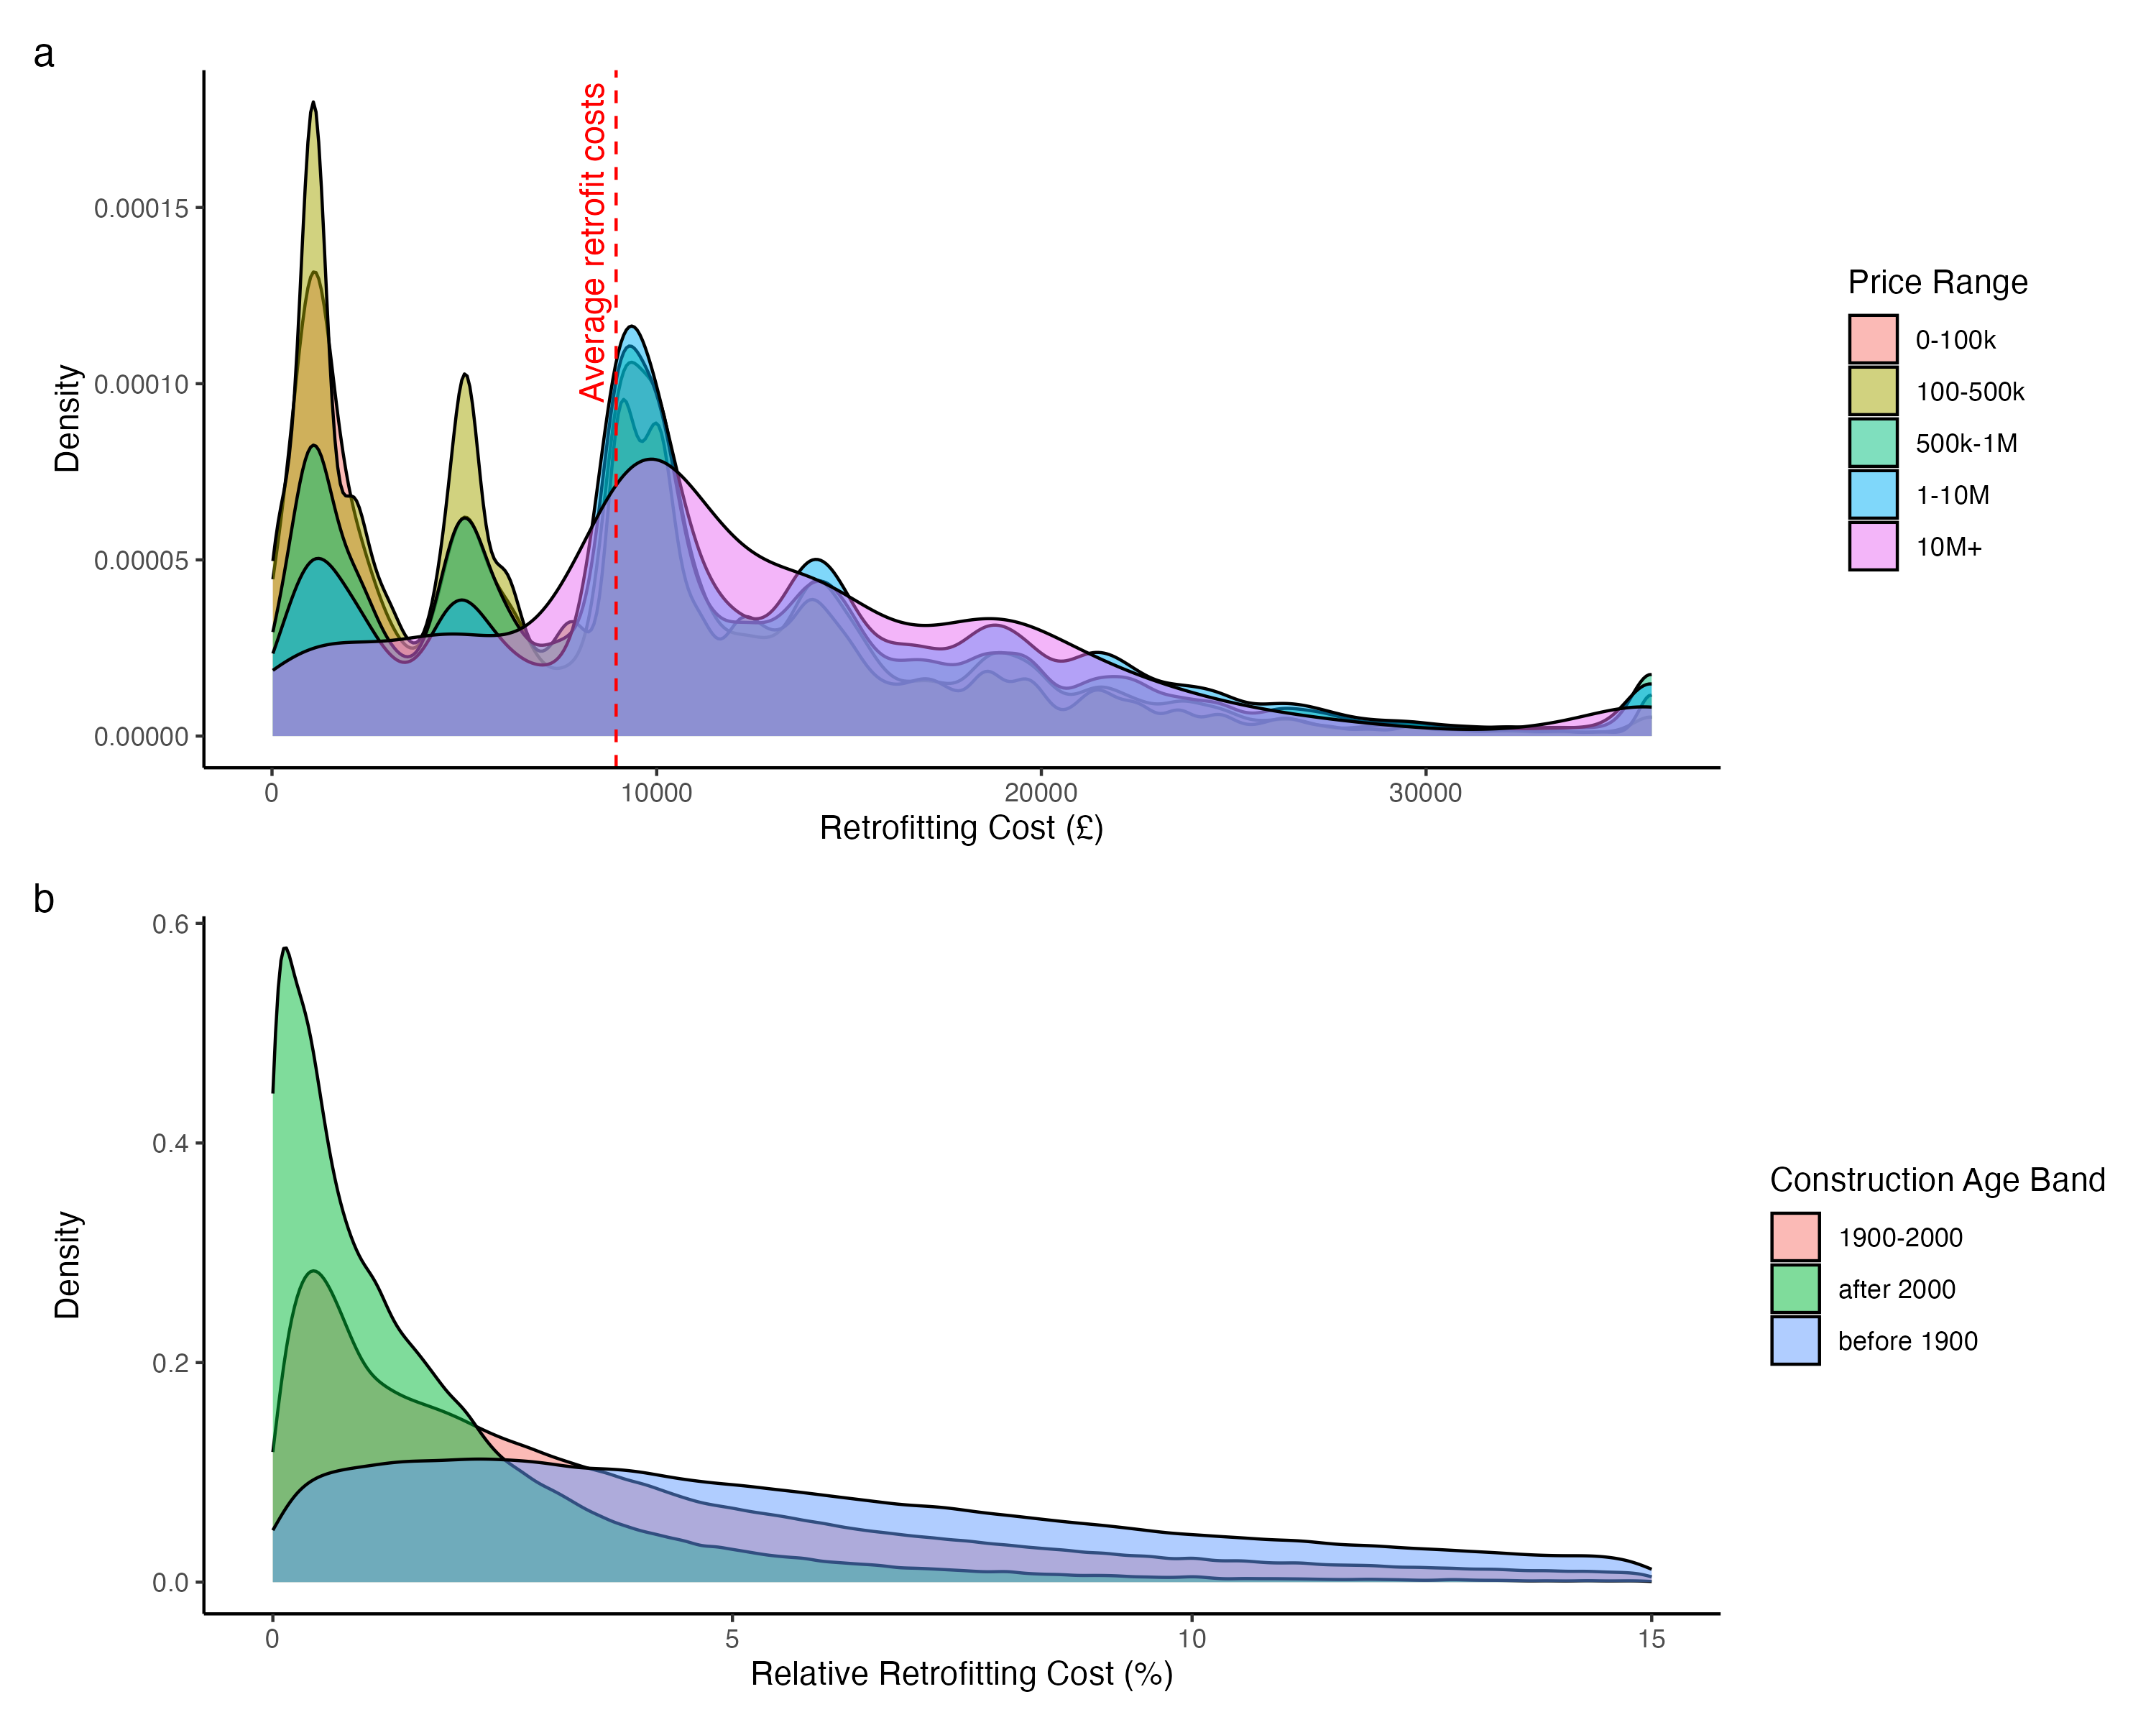
\includegraphics[width=1\linewidth]{src/figures/Combined_Density_Costs.png}
    \caption{Density plot of absolute (a.) and relative (b.) household retrofitting costs from following EPC recommendations (Strategy 1) to reach hypothetical MEES of EPC - C. Relative costs were determined as percent of property value as of latest transaction. The dashed line in subplot a. represents the average retrofitting cost per household according to this strategy (\textsterling 9,058 according to Table \ref{EPC_69_costs}). Top 1\% of properties with high retrofitting costs were excluded (winsorized at 99\%) to avoid outliers.}
    \label{fig:density_plot}
\end{figure}

\noindent While an estimate $15.6 $ million registered dwellings were considered 'able to improve their energy efficiency' according to their EPC \footnote{A dwelling considered 'able to improve' here refers to EPCs including improvement recommendations and a differing potential energy efficiency as outputted by the SAP software. } , $6$ million observations had above-standard energy efficiencies and $1$ million properties were unable to every reach a minimum C-Band energy rating (EPC Score of 69) as their 'potential energy efficiency' fell below such threshold. According to the 2015 Energy Efficiency Regulations, dwellings unable to meet MEES require to retrofit until reaching full energy efficiency potential or spending above the a maximum retrofitting budget set by the government. Retrofitting costs the all properties were then computed analogous methodologies and summarized in Table \ref{tab:table5_costsdescription}. 

% add unable to improve at all, and unable to spend at least 10k?
\begin{table}[h!]
\centering
\caption{Dwellings of various capacities to reach the potential MEES of EPC - C. }
\label{tab:table5_costsdescription}
\resizebox{\textwidth}{!}{ 
\begin{tabular}{lrrr}
\toprule
& \textbf{Already Achieved} & \textbf{Unable to Reach} & \textbf{Able to Reach EPC 69} \\
\midrule
\textbf{Number of Houses} & 6,368,752 & 1,060,889 & 8,171,825 \\
\textbf{Total Retrofit Costs} ($10^9$\textsterling) & - & 9.4 & 8.3 \\
\textbf{Reduced Emissions} ($MtCO_2{eq}/yr$) & - & -1.7 to - 2.0 & -12.8 to -20.6 \\
\addlinespace
\textbf{Average Retrofit Cost (\textsterling)$^*$} & - & 8,571 & 9,058 \\
Avg. \textit{pre-}retrofit EPC & 75 & 48 & 57 \\
Avg. \textit{post-}retrofit EPC & - & 61 & 69 \\
\addlinespace
\textbf{Average Property Price (\textsterling) } & 290,397 & 327,014 & 287,725 \\
\bottomrule
\end{tabular}
}
\begin{minipage}{\textwidth}
\scriptsize{\textit{\small{\textbf{NOTE: } For properties unable to reach EPC - C, retrofit costs were determined from maximum energy efficiency potential.}}}
\end{minipage}
\end{table}





\subsection{Green premium for energy efficiency} \label{Sec:green_premium}

\textbf{Green premium: 3 confounders (demand, supply and renovations/condition of the house at time of sale) we add interest rates, and listing data to take care of most important factors. 
need one more column with both interest rate and listing data.
listing were aggregated/counted active per area around a property 30 days (TBD) before transaction finalised as it takes an average of 3 months to complete.}

A  hedonic regression model was used to reveal the marginal effects of energy efficiency and other building characteristics at the time of sale on the transaction price. Hedonic price model was used to estimate willingness to pay using transaction price data \cite{harrison_hedonic_1978} using an adjusted OLS regressions of deflated prices ($P_{it}$ ) as a function of  the SAP score and attributes extracted from the EPC data ($X_{it}$):

\begin{align}
    \text{P}_{it} = \alpha_i + \beta_1 \cdot \text{EPC}_{it} + \sum_{j=2}^{8} \beta_j \cdot             \text{X}_{j,it} +  \gamma_t \cdot \text{time}_t + \epsilon_{it}
\label{Hedonic_m2}
\end{align}

Where \(\beta_{1:9}\) are the hedonic weights and $X_{it}$ are comprised of the total floor area ($X_2$), property type ($X_3$), number of habitable rooms ($X_4$), extension count ($X_5$),, building type ($X_6$), construction age band ($X_7$), and main fuel source ($X_8$) for each dwelling. These are included are control variables to limit omitted variables bias and improve the accuracy and  validity of the model \cite{wilms_omitted_2021}. $\epsilon_{it}$ refers to the standard error terms and, due to the large amount of transactions, is expected to follow a normal distribution. \\
Given that the total floor area is used in the SAP methodology to determine energy efficiency ratings \cite{bre_group_standard_nodate}, it is suspected to be correlated with energy efficiency, there is a concern of multicollinearity and endogeneity. Such concerns are also raised for construction age as part of the key determinants of energy demand, hence ultimately reflected in SAP ratings \cite{hamilton_energy_2013}. This correlation might inflate the estimates and obscure the true relationship between each variable and transaction price.  However the we assume the SAP methodology to take into account this step and provide the EPC ratings as 'fitted' values from building properties. Similarly, ages of dwellings have proven to be significantly correlated to energy efficiency as most houses built after 2012 are much more likely to be energy efficiency \cite{office_for_national_statistics_age_2022}. These potential sources of bias must be considered and taken into account when interpreting the regression results therein. \\

the hedonic price models were executed as OLS regressions using the \texttt{feos} plackage in R \cite{bergman_reframing_2020, berge_efficient_2018} on $10.4$ million transactions. The regressions results are displayed in table \ref{tab:hedonic_model}.  In line with expectations, the analysis reveals that energy efficiency is a statistically significant predictor of transaction price (p-value \textless 0.0001). In the simple hedonic model (Table \ref{tab:hedonic_model}), the coefficient associated with energy efficiency indicates a positive impact on transaction price, with an estimated hedonic premium of approximately £486.72 for every additional improvement in the Energy improvement score. Since the average improvement in energy efficiency across all properties is of 15, the estimates therein would result in an average net green premium of \textsterling $7,331.85$. This suggests that homes with higher energy efficiency ratings tend to command higher prices in the housing market, likely reflecting buyers' willingness to pay \cite{ghosh_homebuyers_2024}. \\

\begin{table}[ht]
\centering
\caption{Regression Results: Hedonic Price Models with Fixed Effects}
\resizebox{\textwidth}{!}{ 
\begin{tabular}{l c c c c}
\toprule
\toprule
& \textit{Simple Hedonic Model}  & \textit{Hedonic Model FE}  & \textit{With Interest Rates}  & \textit{With Listings} \\
\textit{Independent Variable}         & (1) & (2) & (3) & (4) \\
\midrule
Energy Efficiency & $500.88^{***}$ & $486.85^{***}$ & $483.26^{***}$ & $408.46^{***}$  \\
                  & $(5.54)$       & $(5.57)$       & $(5.56)$       & $(7.92)$        \\
\addlinespace
\midrule
Adj. R-Square     & $0.37$         & $0.37$         & $0.37$         & $0.45$          \\
N                 & $8,923,015$    & $8,923,015$    & $8,923,015$    & $4,001,425$     \\
\addlinespace
\midrule
Total Floor Area          & \textit{Yes}    & \textit{Yes}    & \textit{Yes}    & \textit{Yes}    \\
Property Type             & \textit{Yes}    & \textit{Yes}    & \textit{Yes}    & \textit{Yes}    \\
Number of Habitable Rooms & \textit{Yes}    & \textit{Yes}    & \textit{Yes}    & \textit{Yes}    \\
Extension Count           & \textit{Yes}    & \textit{Yes}    & \textit{Yes}    & \textit{Yes}    \\
Built Form                & \textit{Yes}    & \textit{Yes}    & \textit{Yes}    & \textit{Yes}    \\
Construction Age Band     & \textit{Yes}    & \textit{Yes}    & \textit{Yes}    & \textit{Yes}    \\
YEAR Time-Fixed Effects   & \textit{No}     & \textit{Yes}    & \textit{Yes}     & \textit{Yes}     \\
MONTH Time-Fixed Effects  & \textit{No}     & \textit{Yes}    & \textit{Yes}     & \textit{Yes}     \\
Monthly Interest Rates    & \textit{No}     & \textit{No}     & \textit{Yes}    & \textit{Yes}     \\
Active Listings           & \textit{No}     & \textit{No}     & \textit{No}     & \textit{Yes}    \\
\bottomrule
\bottomrule
\addlinespace
\end{tabular}
}
\begin{minipage}{\textwidth}
\scriptsize{\textit{\scriptsize{{\textbf{NOTES:} These estimates are the results of OLS regressions. The table reports the effect of energy efficiency score (out of 100) on property transaction prices (dependent variable). The coefficients represent the change (in \textsterling) in the dependent variable (price) per unit change in the independent variable (energy efficiency). The first column reports the results for the simple hedonic model without time fixed effect and the second column includes the time fixed effects. Regressions include household fixed effects, along with time controls in the second column. Columns (3) and (4) use monthly interest rates and average yearly sale listings by region as fixed effects, respectively. Robust standard errors in parentheses. Significance levels are indicated as $^{***}p<0.001$; $^{**}p<0.01$; $^{*}p<0.05$.}}}}
\end{minipage}
\label{tab:hedonic_model}
\end{table}


When accounting for time-varying controls through the use of other fixed effects, namely monthly interest rates and number of properties listed for sale in the same region, the estimate is reduced to approximately £207.80 (Table \ref{tab:hedonic_model}). The reduction in the coefficient suggests that the initial model may have overestimated the impact of energy efficiency by not accounting for unobserved, unit-specific characteristics that do not vary over time. When controlling for the supply of housing (measured by the number of listings), the adjusted $R^2$ value increased significantly compared to the other models. This improvement in the model's explanatory power underscores the importance of controlling for a broad range of factors that influence housing prices, beyond just energy efficiency. \\


\subsection{Elasticity of supply}
For this the sale price elasticity were parametrically estimated from the given active listings dataset \footnote{Zoopla Limited, © 2024 2. Zoopla Limited. Economic and Social Research Council. Zoopla Property Data, 2024 [data collection]. University of Glasgow - Urban Big Data Centre} from the equation below, similar to work done by \cite{malpezzi_long-run_2001}. Price elasticity refers to the effects of additional demand shocks on residential market prices and draws from the economic theory of "law of demand" \cite{fibich_dynamics_2005}.
\begin{align*}
    ln(P_i) = \beta \cdot ln(\text{active listings}_i) + \gamma_i \cdot t + rent_i : t_i
\end{align*}

According to the properties at risk and potential decision framework to sell or rent therein, over $500$ thousand properties risk entering the housing market for sale.\footnote{all properties with construction age before 1949 and in districts with high retrofitting cost and high fuel-poverty (nealry 2.6 million) and adjusted for the estimated 19\% of dwellings for rent} These refer to homes current renting that may be forced to sale faced with imposed MEES. This may have significant impacts on the UK housing market. According to the results (table \ref{table:coefficients}) elasticity is significant and is estimated that for every additional 1\% in active listings, property prices decrease by 2\%. Since about 8.1 million properties were currently listed in the market (from dataset), an additional 6.3\% properties might enter the market as a result of the MEES. Inducing a 11.3\% drop in property prices.
\begin{table}[ht]
\centering
\caption{Regression results showing the effects of base rate and other predictors on ln of growth\_price.}
\resizebox{0.3\textwidth}{!}{ 
\begin{tabular}{@{}l c@{}}
\toprule
\toprule
\textit{Independent Variables} & \textbf{House Price (\textsterling)} \\
\midrule
\addlinespace
\textbf{ln Active Sales}            & $-0.02^{**}$  \\
                                     & $(0.00)$      \\
\addlinespace                            
Interest Rates             & $0.02^{*}$    \\
                                     & $(0.01)$      \\
\addlinespace
Ajd. Interest Rates              & $-0.01^{*}$   \\
                                     & $(0.00)$      \\
\midrule
N.                    & $3,359,780$   \\
R$^2$        & $0.03$        \\
Adj R$^2$      & $0.01$        \\

\midrule
Property Type & \textit{yes}         \\
District   & \textit{yes}         \\
Year   & \textit{yes}       \\
Month       & \textit{yes}         \\

\bottomrule
\addlinespace    
\end{tabular}
}
\begin{minipage}{\textwidth}
\scriptsize{\textit{\scriptsize{{\textbf{NOTES:} These estimates are the results of OLS regressions. The table reports the effect of supply (number of active sales) on property transaction prices (dependent variable). Robust standard errors in parentheses. Significance levels are indicated as $^{***}p<0.001$; $^{**}p<0.01$; $^{*}p<0.05$.}}}}
\end{minipage}
\label{table:coefficients}
\end{table}


While the estimates above represent an immediate effect of the induced supply shock, which will inevitably decrease with time \cite{fibich_dynamics_2005}, it is highly significant. The increased supply of homes may have direct effects on the local housing prices but also have knock-on effects on neighbouring regions which buyers consider subsitutable \cite{fingleton_housing_2019} . This may have implications on the current housing crisis by increasing the supply of homes and potentially increase affordability across the UK.
\section{Discussion}

Note: similarly no impact on rental market (as rents are always at max capacity). The ogernment should focus on insulation. we also need to distinguish between all homes and rental properties when mentioning the figures below. Are the cost tables 3, 4 and 5 for all properties or just rentals? (we will need both).


Imposing a stricter energy efficiency standard (MEES) of 69 on all dwellings capable of reaching such standards has the potential of decreasing the UK's housing annual emissions by 38.2-42.5\% from 2022 levels \footnote{values determined from EPC retrofitting strategy for both houses able and unable to reach 69.} (and 52.3 - 55.6\% from 2017 baseline levels) \cite{department_for_business_energy_and_industrial_strategy_english_2023, department_for_business_energy_and_industrial_strategy_household_2020, office_for_national_statistics_energy_2023}.  If $8.2$ million properties retrofit to an EPC of C within 2028 - as recommended by the CCC \cite{climate_change_committee_ccc_2022_2022} - the UK housing sector would surpass its NZ targets of decreasing 50\%  of  residential emissions by 2032 compared to 2017 \cite{department_for_business_energy_and_industrial_strategy_english_2023}. The UK could be well on the road to Net Zero. While setting MEES could serve as a critical pathway for England and Wales to meet their Net Zero goals by 2050, the success of the policy amendment must be weighed against the financial incentives for households and the broader impacts on the already challenging domestic housing sector. \\

Households across England and Wales would have to bear a cost of \textsterling $91.6$ billion \footnote{This figure includes \textsterling 82.5 to reach an EPC of C and \textsterling9.1 for all other dwellings to reach their maximum energy efficiency potential.} in energy improvements  to reach a minimum EPC standard of C (score of 69 out of 100) - or at least maximum efficiency potential with the current ceiling. Results indicate over \textsterling 29 billion would be spent on wall insulation (ID 7), followed by \textsterling 13 billion in solar water heating technologies (ID 19). The overall costs of these two technologies have not significantly come down in recent years, sitting at \textsterling10,000-9,000 and \textsterling 5,000 - respectively. These were possibly induced by a lack of demand and 'experience learning-curve' effect \cite{lafond_how_2018, zhou_learning_2019, bosetti_witch_2006} as uptake of solar water heaters and wall insulation measures had remained low in the past - despite government incentives and EPC recommendations \cite{hamilton_uptake_2014}. The average retrofitting cost at household level of 
reaching MEES ranges from \textsterling 6,434 to \textsterling 10,000 based on three different retrofitting strategies. However, as with aggregate costs, such prices may be overestimated as experiential learning curves and economies of scale have not been taken into consideration \cite{lafond_how_2018}. Should households commit to retrofits as suggested in their EPC reports, the resulted cost would be higher than identifying the most impactful retrofits with respect to price per price. 

This is concerning as property owners have limited information when deciding to commit to green retrofits and other geographical and time dependent factors are likely to influence this decision as well, including the potential rent premium for higher efficient properties or the surcharge paid for a property due to lack of supply, thus exacerbating inequalities. Landlords might simply decide to sell their rental properties as future rents would not be able to compensate for the upfront costs associated with meeting the new EPC and the loss of rents while retrofits are being conducted. \\


The average retrofitting costs of achieving minimum energy efficiency of 69\% - or highest energy efficiency potential for less-able properties -  vary widely by construction age and price range. Older properties, especially pre-war homes, would have to incur higher retrofitting costs due to their low efficiency. These account for over 35\% of properties in the UK and Wales, with wales having more very old homes \cite{building_research_establishment_housing_2018}. Property owners would have to spend  \textsterling 9-15k in renovations for those able to reach 69\% and \textsterling 8-10k for others to reach their maximum energy efficiency. \\

\begin{figure}[ht]
    \centering
    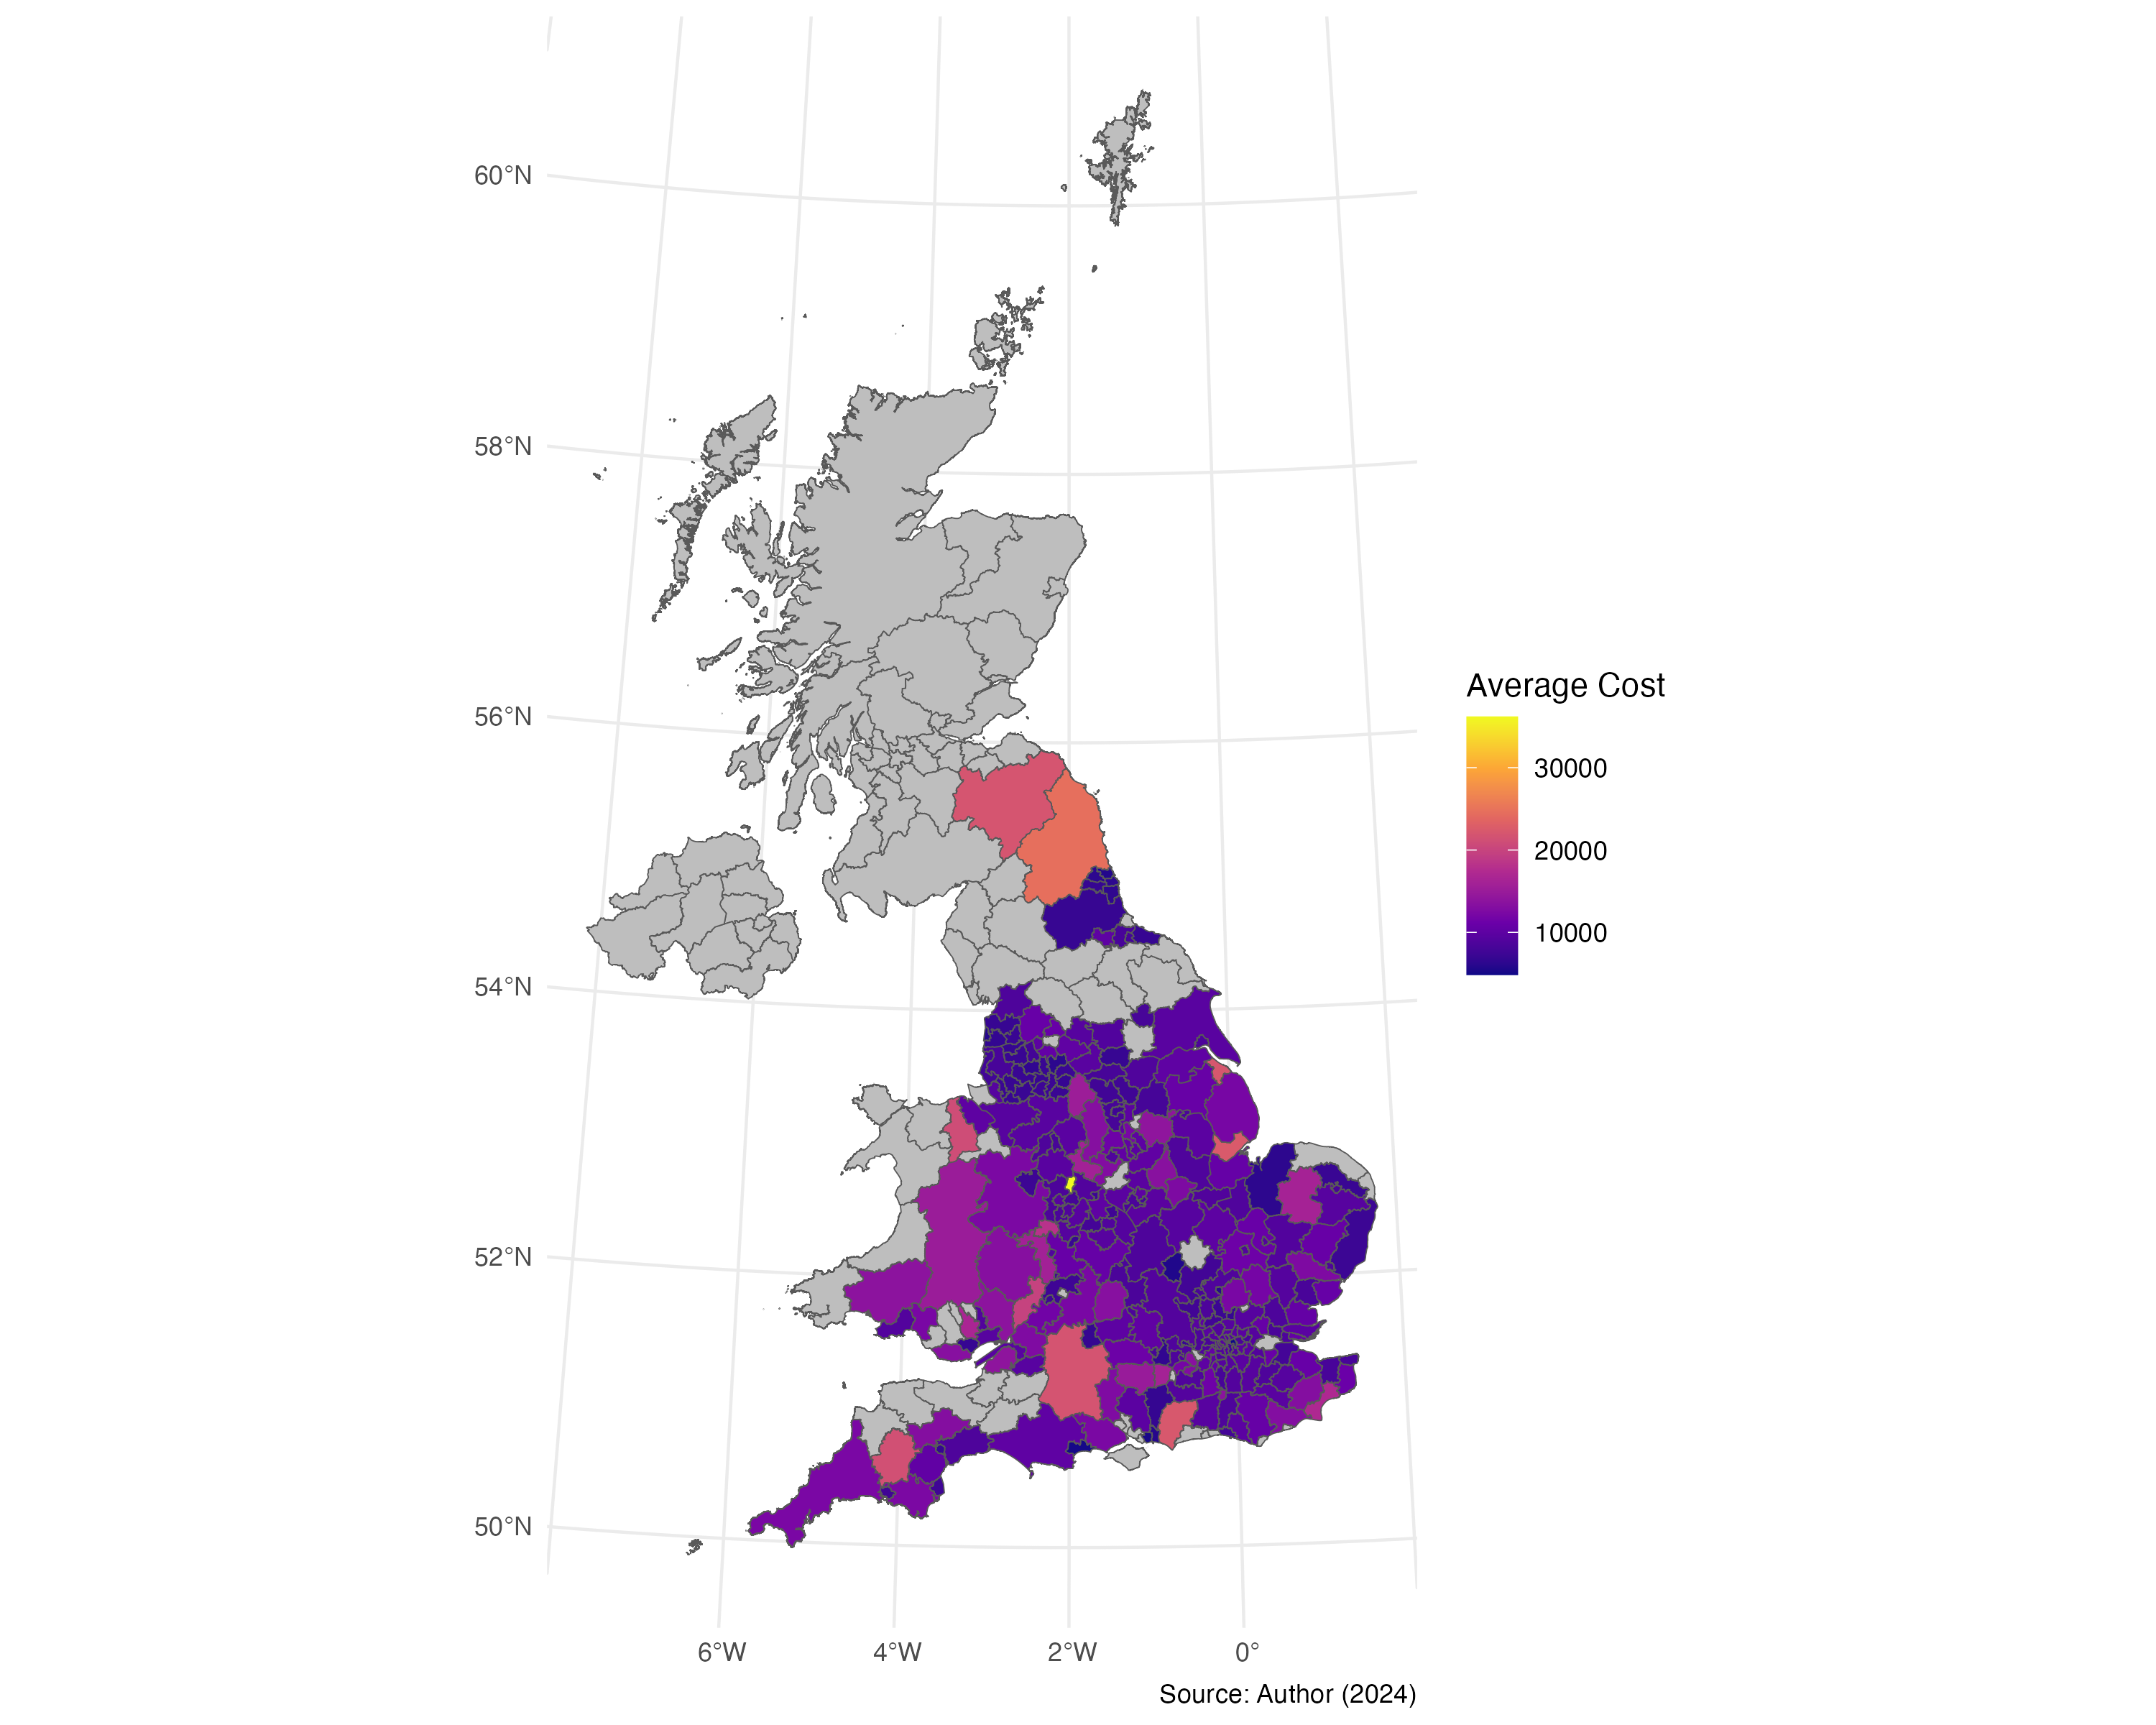
\includegraphics[width=1\linewidth]{src/figures/average_costs_per_district.png}
    \caption{Average retrofitting costs per district in England and Wales (sourced shapesfiles from ONS)}
    \label{fig:costs_district}
\end{figure}

Although not highly geographically heterogeneous (Figure \ref{fig:costs_district}), certain districts seem to show above-average retrofitting costs to reach the new requirements. These correspond to the local authority districts of the Scottish Borders, Northumberland in the Northeast as well as Wiltshire and West Devon in SouthWest which are largely rural  \cite{vera-toscano_ruralurban_2024}. These align with existing reports of unusually high poverty in these districts \cite{baker_profile_2003, scottish_borders_council_lhs_2016}. Fuel poverty is often associated with low income and less-energy efficient households as affordability for energy costs are low \cite{baker_predicting_2003}.


Although the figures therein represent the estimated costs as houses implement recommendations from the EPCs, there is no legal requirement for property owners to follow such order. Instead, a minimum energy efficiency standard - as suggested by the UK government in 2021 - would take a 'whole house retrofit' approach and not take into account the nuances of property-level decisions. However, as seen by the nuances and sensitivity of the costs by retrofitting strategy (\ref{EPC_69_costs}), an surgical approach to retrofitting would capture much more nuances to overall retrofitting costs and total abated emissions \cite{alabid_review_2022, uk_green_building_council_ukgbc_retrofit_2021}.\textbf{ }Indeed, the results confirmed previous studies' criticism on the energy-cost focused narrative of the SAP and RdSAP recommendations \cite{kelly_building_2012} . A more sequential and tailored approach to implementing energy efficiency improvements, prioritizing those with the highest yield, could significantly reduce household costs and facilitate more coordinated investments in specific improvement industries, potentially driving down retrofitting expenses \cite{alabid_review_2022}. As previously discussed, the EPC retrofitting scheme designed to meet the Minimum Energy Efficiency Standards (MEES) has emphasized investments in technologies that are individually expensive and have not demonstrated significant price reductions over time. In contrast, if households were to prioritize improvements that offer the greatest efficiency gains relative to their cost, the majority of aggregate spending would likely be directed towards the installation of solar photovoltaic (PV) panels (ID 34). Such large-scale investment—potentially exceeding £16 billion—could, over time, further reduce retrofitting costs for homeowners as the increasing adoption of PV technology drives economies of scale and fosters technological advancements \cite{lafond_how_2018}. Effective policies in the past have proven to possible to positively affect industry prices and end-user implementation of green innovations.  Indeed, uptake of biogas in countries like India and China have increased as a result of up-to-date policy initiatives \cite{abanades_critical_2022}. Therefore, an effective and demographically tailored regulation on retrofitting schemes would significantly decrease household renovation prices for households while also enabling focused investments green technologies. Further decreasing prices and enabling more properties to reach higher energy efficiencies by reducing financial limits to MEES and making EPC C potentially more affordable under an elemental approach. \\

Only 29\% of retrofitting costs would fall below current energy retrofitting household spending of \textsterling 3,500 as currently implemented by the Private Renting Energy Efficiency Regulations  \cite{department_for_energy_security_and_net_zero_and_department_for_business_energy__industrial_strategy_standard_2023}. Hence, as suggested by the 2021 amendment proposal \cite{department_for_energy_security_and_net_zero_desnz_and_department_for_business_energy_and_industrial_strategy_beis_heat_2021}, an increase in household spending budget would be required to require the desired number of properties to reach an EPC of C. policy makers should consider tailoring this threshold  by property type and construction age. According to the aggregated results therein, the marginal abatement costs for residential emissions can be derived and is estimated at \textsterling 3,273 to \textsterling5,124 per tonne of $CO_2$. This is significant compared to system-wide abatement costs estimated from changing fuel-source of the UK electricity grid \cite{mckinsey_company_appendix_2002}. Suggesting placing all retrofitting costs on end-users to be less efficient than a universal carbon tax to decarbonize the grid and highlighting the importance of introducing system-wide policies in parallel to increasing MEES. 


Several limitation underpin the findings and recommendations suggested above. First, EPCs have been proven as better estimators of energy cost-efficiency \cite{kelly_building_2012}and tend to overestimate energy use \cite{few_over-prediction_2023}. Therefore, more accurate indicators of energy use such as meter data would be preferable to assess post-retrofitting reductions in energy usage. Second, certain types of retrofits are more intrusive than others and require longer installation times resulting in higher costs, further disinventing landlords to commit to these in fear of loss of rental income. Third, the green premium was estimated using a hedonic price model which suffers from different confounding factors, such as demand and supply forces surrounding the point of sale which could result in overestimating the green premium associated with green retrofits. This however provides a ceiling for the estimates in this study. Last, green retrofits might be less costly when committed together as installation costs were computed assuming independent deployment. Improvements, such as cavity wall installations, have also shown not to have long-lasting effects on energy efficiency \cite{penasco_assessing_2023}. By not taking into account such time-varying effects the estimated gains from future energy savings might be overestimated. \\

Future research may want to look further into each aspect of the effects induced by imposed MEES. These may include looking at the specific improvements undertaking by household characteristics and demography to better understand the national-scale investments needed to deploy effective retrofitting strategies. Additionally, while this study could not rely on tenure statistics for more granular estimates, a deeper understanding of the underlying decisions to resale may provide further insights into the market shock produced by imposed standards. Limitations of time and processing power prevented this study from other more robust methods of isolating the effects of certain energy improvements. A potential avenue for investigating such trends would have been to use propensity-score matching (PSM) across properties of similar attributes \cite{fuerst_does_2015, fuerst_energy_2016, penasco_assessing_2023, zhang_price_2017, zhang_does_2021}. \\

To be honest I feel that computing a cost of abatement reveals troubling figures, i.e. the cost per ton of carbon avoided is super high... one conclusion would be that it is much cheaper to decarbonise the grid instead, even if the price of electricity increases drastically it nowhere in the region of what a household would pay. this in itself would be incentive enough to focus on the deployment of renewables. boiler upgrade scheme is 7.5k for gov so how many tons avoided from this once you add up consumer costs? (I can give an asnwer from MCS data BTW)







\section{Conclusion}

At the national level, mandating improvements in energy efficiency could be pivotal in enabling the UK to meet its Net Zero goals by 2035. The analysis reveals that large-scale investments in photovoltaic (PV) panels, as well as advanced heating and hot water technologies, would be essential for compliance. However, by adopting a strategic approach that leverages learning-by-doing and targeted investments, the UK could substantially reduce the financial burden associated with these upgrades. The study found significant variability in the estimated costs of meeting the proposed energy standards, indicating that more refined and well-communicated strategies could improve the effectiveness and uptake of energy performance improvements beyond the current RdSAP outputs on Energy Performance Certificates (EPCs). \\


The research corroborates existing empirical evidence on the existence of a green premium for enhanced energy efficiency on property values. While improving properties to an EPC rating of C is likely to have net-positive effects on both property values and energy savings, these benefits must be weighed against the substantial costs of retrofitting. These costs vary significantly depending on the age of the property and fuel poverty in a given area as for older and rural dwellings with low energy efficiency, retrofitting costs would exceed government budgets, impeding the financial viability of these investments. Consequently, landlords of privately rented properties may find it more financially prudent to sell rather than risk exposure to unstable energy and rental markets. The study estimates that approximately 500,000 properties could be at risk of sale due to these pressures, potentially triggering an 11\% decline in housing prices within the UK market. \\

The findings of this study suggest threefold benefits of implementing a minimum EPC rating policy as this single policy could lead to sectoral emissions reductions, create green premiums for homeowners, and induce a significant correction in housing prices. While this could potentially help alleviate the current housing crisis, further research is needed to estimate the drivers behind the decisions of committing to green retrofits and the extent to which certain technologies, such as solar PVs and heat pumps, could bring combined benefits for property owners. A minimum EPC C standard for privately rented homes in England and Wales, when combined with grid-wide decarbonization strategies and tailored subsidy programs, could serve as a comprehensive 'triple-win' strategy, effectively harnessing market dynamics to achieve environmental, economic, and social benefits.


% Appendices
\appendix
\section{Additional Results}
\label{appendix:results}
\input{src/sections/appendix}

% Bibliography using natbib (compatible with elsarticle)
\bibliographystyle{elsarticle-num}
\bibliography{references.bib}

\end{document}